\chapter{Introduction}
Universal Serial Bus (USB) is the most widely-used connector for modern computer systems. It allows various devices to connect to the computer. The USB has replaced many older interfaces, such as parallel and serial ports, and has become the standard for connecting devices such as keyboards, mice, printers, and storage devices to computers. The main selling point of the USB interface was the introduction of "plug-and-play" feature which removes the need for the users to configure the device. Upon connecting the device to the computer, the system automatically recognizes the device and immediately assigns appropriate drivers.

Unfortunately, as the popularity of the interface grew, new types of malicious attacks against USB began to emerge. In 2014, a group of researchers from Security Research Labs announced a new type of USB malware called BadUSB. They demonstrated a USB device with modified firmware that could spoof a keyboard, network card, and even a display. And this type of malware is undetectable by conventional antivirus programs.

The main focus of this work is to design and implement this type of device on the Raspberry Pi Pico board, as well as to evaluate what the finished product is capable of. There are numerous defense mechanisms that have been created since the introduction of the malware. So I put my device to the test against several of them to see how it performed.

The aim of this thesis is to provide readers with an overview of the BadUSB attack security issue so that they can better understand what makes them so dangerous, how they work and how to defend against them. My implementation therefore gives readers a low-cost and simple means to experiment with BadUSB device.

\chapter{Universal Serial Bus}
\label{usb}
Universal Serial Bus (also known as USB) is a peripheral interface used to connect external devices to computers. It defines the specifications of cables, sets of protocols, the speed of data exchange, and the way the host and device communicate with each other. Not only that, but it can also send power to devices (for example to charge smartphones).

Before the invention of the USB peripheral, there exists countless kinds of ports in any shape and size. In the past, every peripheral has its shaped connector, a protocol through which it communicated with the computer, and a limited number of devices it can run at once. And that brings many disadvantages.

First of all computer manufacturers had to decide which sets of ports to include in the final motherboard. We can usually find ports like PS/2 for connecting keyboards and mouses, or VGA connectors for connecting monitors on the old machines. But what if the user wanted to connect a device (for example a scanner or a printer), whose port simply wasn't included with the machine? They usually had to go out and purchase dedicated cards and then manually install them. That is something a person without computer experience might have struggled with. And as for developers during the development of new computer accessories, they had to decide whether to use one of the existing interfaces but run into a risk of being stuck with its original protocols that don't provide enough features the developer needs or design a new interface which is very expensive.

That led to the development of a new interface. In 1995 a group named \textbf{USB Implementers Forum} (also known as USB-IF) was formed by these seven companies: Compaq, DEC, IBM, Intel, Microsoft, NEC, and Nortel. They aimed to create an interface with these goals in their mind:
\begin{itemize}
    \item \textbf{Easy to use} \--- The user doesn't need to configure and set up a device.
    \item \textbf{Fast} \--- To minimize the delay in communication between the host and device and to be able to transfer
    \item \textbf{Reliable} \--- To minimize the occurrence of errors and automatic error handling.
    \item \textbf{Versatile} \--- Many kinds of peripherals can use the interface.
    \item \textbf{Inexpensive} \--- So that the price of a final product can be as low as possible.
    \item \textbf{Supported by all operating systems} \--- It helps developers to write the drivers for the peripherals.
\end{itemize}

A year later, USB-IF released the first version of the USB interface called \textbf{USB 1.0}. The new interface allowed a user to connect a variety of peripherals, such as printers, keyboards, mobile devices, and much more, using a single, standardized interface socket. It also lets the user connect and disconnect a peripheral whenever needed without needing to shut down a computer. And at last, a feature called "plug-and-play" was introduced. It shows the simplicity of the USB \--- the user simply plugs the device into the computer and can immediately use it.

But it wasn't until the introduction of \textbf{USB 1.1} in 1998 that the interface started to be widely used. In that year the operating system Windows 98 was shipped together with support for USB. Version 1.1 also introduced two speeds: Low Speed with 1.5 Mbps and Full Speed with 12 Mbps.

Over the next 20 years, USB has been constantly upgraded. In April 2000 \textbf{USB 2.0} was released and with it a new maximum transfer rate of 480 Mbps. It was called High Speed. Eight years later in November 2008, USB-IF released a new specification for \textbf{USB 3.0} with an even faster transfer speed of 5 Gbps (named SuperSpeed USB). As for the time of writing this thesis USB-IF has released the specification for \textbf{USB4 2.0} with a maximum transfer rate of 80 Gbps and power delivery of 240 W (48 V, 5 A).

Nowadays almost every device is equipped with some form of USB either for charging or data transfer. From smartphones and game consoles to microcontrollers and soldering iron. And there are currently 14 different types of USB connectors (some of them are shown in \autoref{fig:usb_connectors}, Type-C being the latest one introduced in December 2013.

\begin{figure}[ht]
    \centering
    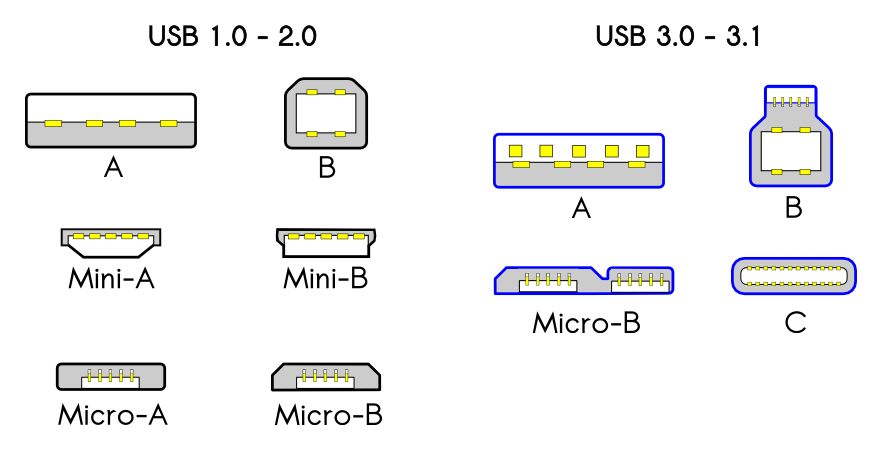
\includegraphics{./obrazky-figures/USB_connectors.png}
    \caption{List of mostly used USB connectors per generation}
    \label{fig:usb_connectors}
\end{figure}

\subsection*{Communication between Host and Device}
\label{communication}
The standard USB interface has four signal lines and two of those are used to carry data from all of the devices. As seen in \autoref{fig:usb_pins}, the lines are \textbf{Vcc} for the power, \textbf{GND} as ground, and \textbf{D+} and \textbf{D-} for data transfer. Unlike UART, where it uses Rx data line for receiving data and Tx for transferring data, USB uses both wires to carry a single differential signal. Directions are taking turns.

\begin{figure}[ht]
    \centering
    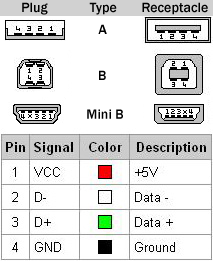
\includegraphics{obrazky-figures/usb_pinouts.png}
    \caption{USB pin layouts}
    \label{fig:usb_pins}
\end{figure}

Before a transfer between the host and devices starts they have to establish some sort of communication canal. In USB terminology that means to establish a \textbf{pipe}. The pipe connects the host with the device's endpoint. \textbf{Endpoint} is an allocated block of memory or a register on the controller's chip where received data or data waiting to be sent are stored. The host doesn't have an endpoint since it initiates and finishes the transmission. The connection is initiated during the \textbf{enumeration} -- an initial sequence of data exchange between the host and device.

\begin{figure}[ht]
    \centering
    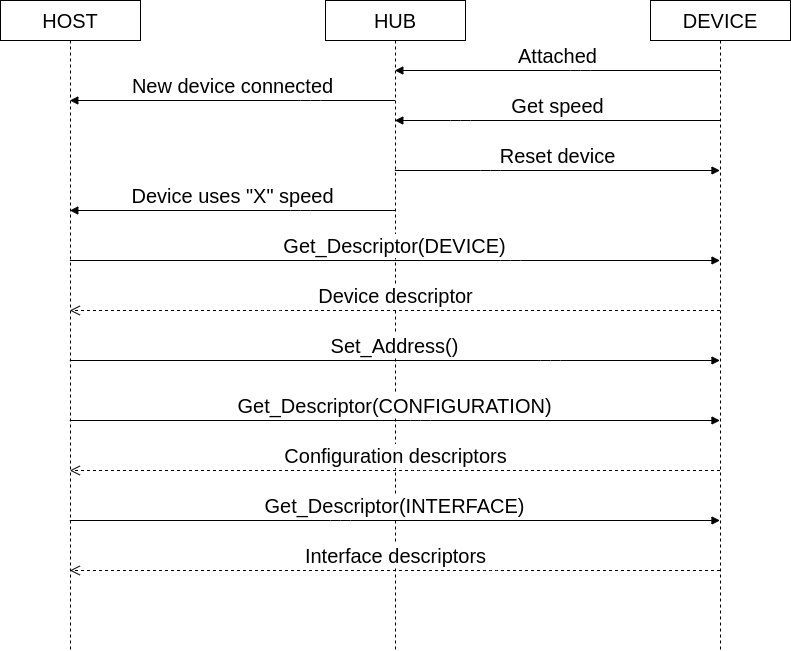
\includegraphics[width=260px]{obrazky-figures/enumeration.png}
    \caption{USB enumeration in sequence diagram}
    \label{fig:enumeration}
\end{figure}

Endpoints are only one-directional, except for control endpoints. The receiver is called \textbf{the sink} and the sender is \textbf{the source}. During the enumeration, the host assigns a unique address for each endpoint defined in the descriptor (more about descriptors in \autoref{descriptor}). The direction is specified in the transaction type which is defined from the host's perspective: \emph{IN} for receiving data (host receives data) and \emph{OUT} for sending data (host sends data). Control (Setup) data must support bidirectional transfer data.

Every device has Endpoint 0 configured for control transfer. It is used by the host to send a request to the device.

\newpage
\begin{table}[ht]
    \centering
    \begin{tabular}{|l|c|c|p{0.39\linewidth}|} \hline
         \textbf{Packet type} & \textbf{PID name} & \textbf{PID value} & \textbf{Description} \\ \hline
         \multirow{4}{3cm}{Token (identifies transaction type} & OUT & 0001 & Device and endpoint address for OUT transaction. \\ \cline {2-4}
           & IN & 1001 & Device and endpoint address for IN transaction. \\ \cline{2-4}
           & SOF & 0101 & Start-of-Frame marker and frame number. \\ \cline{2-4}
           & SETUP & 1101 & Device and endpoint address for Setup transaction. \\ \hline
         \multirow{4}{3cm}{Data (carries data or status code)} & DATA0 & 0011 & Data toggle, data PID sequencing \\ \cline{2-4}
           & DATA1 & 1011 & Data toggle, data PID sequencing \\ \cline{2-4}
           & DATA2 & 0111 & Data PID sequencing \\ \cline{2-4}
           & MDATA & 1111 & Data PID sequencing \\ \hline
         \multirow{4}{3cm}{Handshake (carries status code} & ACK & 0010 & Receiver accepts error-free data packet. \\ \cline{2-4}
           & NAK & 1010 & Receiver can't accept data or sender can't send data or has no data to transmit \\ \cline{2-4}
           & STALL & 1110 & A control request isn't supported or the endpoint is halted. \\ \cline{2-4}
           & NYET & 0110 & Device accepts error-free data packet but isn't yet ready for another or a hub doesn't yet have complete-split data. \\ \hline
        \multirow{5}{3cm}{Special} & PRE & 1100 & Preamble issued by the host to indicate that the next packet is low speed. \\ \cline{2-4}
          & ERR & 1100 & Returned by a hub to report a low- or full-speed error in a split transaction. \\ \cline{2-4}
          & SPLIT & 1000 & Precedes a token packet to indicate a split transaction. \\ \cline{2-4}
          & PING & 0100 & Busy check for bulk OUT and control Write data transaction after NYET. \\ \cline{2-4}
          & reserved & 0000 & For future use. \\ \hline
    \end{tabular}
    \caption{List of Packet ID and their description}
    \label{tab:pid}
\end{table}

There are four types of transfers: Control, Bulk, Interrupt, and Isochronous. Each device can use different types depending on the need. \textbf{Control transfers} enable the host to read information about the device and allow it to configure and update the device's inner status. All USB devices are required to support this type of transfer. \textbf{Bulk transfers} are used in situations where the transfer rate is not critical such as sending a file to the printer or receiving data from the scanner. The priority of the transfer is the lowest. \textbf{Interrupt transfers} on the other hand are implemented in devices where instance feedback is needed. For example, click of a button on the keyboard or a movement of a mouse. \textbf{Isochronous transfers} guarantee delivery of data but no error correction is implemented. Usually used to transfer audio and video in real time. If an error occurs the device doesn't re-transmit lost or corrupted data.

The process of sending data is called \textbf{transfer}. Transfer consists of one or more \textbf{transactions} which are block of packets that starts with \textbf{token packet}. Transaction can also contain additional packets called \textbf{data packet} and \textbf{handshake packet}. Each packet begins with a Packet ID (PID) that specifies what information the packet carries. The list is showed in \autoref{tab:pid}. In the first phase (token phase\footnote{Phase is a part of a sequence of a transaction. There can be three parts named after packets: token phase, data phase and handshake phase}), the host initiates communication by sending a token packet. In data phase, the host or device may transfer any kind of data in the data packet. And in the last (handshake) phase, the host or device sends status information in a handshake packet. There are also four special PIDs only used by low-speed devices.

\subsection*{Descriptors}
\label{descriptor}
USB descriptors are data structures formatted into blocks that contain information about the device. It is used during the enumeration. All USB devices must be able to respond to requests for standard USB descriptors.

There are in total 11 descriptor classes that the device can define but not all of them are required. The list of them is shown in \autoref{tab:descriptor_types}. All descriptor types are identified by their identifier value that is set in \emph{bDescriptorType} field. Each descriptor class consists of a series of fields. There is a standardized naming convention for each field indicating which format of data it contains: \emph{b} is a byte (8 bits), \emph{w} is a word (16 bits), \emph{bm} is a bit map, \emph{bcd} is a binary-coded decimal, \emph{i} is an index, \emph{id} is an identifier. From \autoref{tab:descriptor_types} we can see that three descriptors are required: device, configuration, and interface.

\begin{table}[ht]
    \centering
    \begin{tabular}{|l|l|p{0.39\linewidth}|} \hline
         \textbf{bDescriptorType} & \textbf{Descriptor Type} & \textbf{Required?} \\ \hline
         0x01 & device                      & Yes \\ \hline
         0x02 & configuration               & Yes \\ \hline
         0x03 & string                      & No  \\ \hline
         0x04 & interface                   & Yes \\ \hline
         0x05 & endpoint                    & No if device uses only Endpoint 0 \\ \hline
         0x06 & device\_qualifier           & Only if the device supports both full and high speeds \\ \hline
         0x07 & other\_speed\_configuration & Only if the device supports both full and high speeds \\ \hline
         0x08 & interface\_power            & No \\ \hline
         0x09 & OTG                         & Only for On-The-Go devices \\ \hline
         0x0A & debug                       & No \\ \hline
         0x0B & interface\_association      & Only for composite devices \\ \hline
         \end{tabular}
    \caption{List of descriptor types}
    \label{tab:descriptor_types}
\end{table}

First two bytes of all descriptors stores two important pieces of information: \emph{bLength} declares the size of the descriptor/buffer that the host received and \emph{bDescriptorType} tells the host what type of information can it expect in the buffer.

\textbf{Device} descriptor contains basic information about the device itself such as the version of USB used, device class, manufacture information, number of configurations of the device, and more. It's the first descriptor that is sent to the host. In total, the host will receive a buffer of 18 bytes. After the host retrieves the first descriptor it sends a request for a \textbf{configuration}, \textbf{interface}, and \textbf{endpoint} descriptors. They specify the device's features and abilities.

When developing a device with a version of USB 2.0 or higher some additional data needs to be set. Since this version of USB allowed a developer to choose what transfer speed to use, he also is responsible to define the device information and configuration of the speed not in use. And for that reason, \textbf{device\_qualifier} and \textbf{other\_speed\_configuration} were created. The former contains \emph{device} descriptor of a device whose speed is currently not in use and the same goes for the latter one with \emph{configuration} descriptor.

\textbf{Interface association} descriptor identifies multiple interfaces that are associated with a function\footnote{Function as a USB term is a device that provides a capability for the host (for example a keyboard)}. What that means is that a driver can support multiple interfaces within one device, such as the video and audio interface for a webcam.

\textbf{String} descriptor contains descriptive texts. Other descriptors can address each text using indices. For example, if \emph{iManufacture} is set to \verb|0x03| it tells the host that the name of the manufacturer is stored as the fourth string descriptor.

Other descriptors \--- \textbf{interface\_power}, \textbf{OTG}, \textbf{debug} \--- are not relevant to this thesis and their definitions can be found in the official documentation.

\autoref{tab:list_descriptors} displays the structure of each descriptor. The tables were taken from Chapter 4 of the book called \emph{USB Complete: Everything You Need to Develop Custom USB Peripherals}. \autoref{lst:dsc_example} shows an example of a device descriptor's buffer.

\begin{longtable}{|c|l|c|} \hline
    \textbf{Descriptor Type} & \textbf{Field} & \textbf{Bytes} \\ \hline
    \multirow{14}{*}{device (0x01)} & bLength & 1 \\ \cline{2-3}
      & bDescriptorType & 1 \\ \cline{2-3}
      & bcdUSB          & 2 \\ \cline{2-3}
      & bDeviceClass    & 1 \\ \cline{2-3}
      & bDeviceSubclass & 1 \\ \cline{2-3}
      & bDeviceProtocol & 1 \\ \cline{2-3}
      & bMaxPacketSize0 & 1 \\ \cline{2-3}
      & idVendor        & 2 \\ \cline{2-3}
      & idProduct       & 2 \\ \cline{2-3}
      & bcdDevice       & 2 \\ \cline{2-3}
      & iManufacturer   & 1 \\ \cline{2-3}
      & iProduct        & 1 \\ \cline{2-3}
      & iSerialNumber   & 1 \\ \cline{2-3}
      & bNumConfiguration & 1 \\ \hline
    \multirow{8}{*}{configuration(0x02)} & bLength & 1 \\ \cline{2-3}
      & bDescriptorType & 1 \\ \cline{2-3}
      & wTotalLength    & 2 \\ \cline{2-3}
      & bNumInterfaces  & 1 \\ \cline{2-3}
      & bConfigurationValue & 1 \\ \cline{2-3}
      & iConfiguration  & 1 \\ \cline{2-3}
      & bmAttributes    & 1 \\ \hline
    \pagebreak \hline
    \textbf{Descriptor Type} & \textbf{Field} & \textbf{Bytes} \\ \hline
      configuration(0x02) & bMaxPower       & 1 \\ \hline
    \multirow{3}{*}{string(0x03)} & bLength & 1 \\ \cline{2-3}
      & bDescriptorType & 1 \\ \cline{2-3}
      & bSTRING/wLANGID & 1/2 \\ \hline
    \multirow{9}{*}{interface(0x04)} & bLength & 1 \\ \cline{2-3}
      & bDescriptorType & 1 \\ \cline{2-3}
      & bInterfaceNumber & 1 \\ \cline{2-3}
      & bAlternateSetting & 1 \\ \cline{2-3}
      & bNumEndpoints   & 1 \\ \cline{2-3}
      & bInteraceClass  & 1 \\ \cline{2-3}
      & bInteraceSubclass  & 1 \\ \cline{2-3}
      & bInteraceProtocol  & 1 \\ \cline{2-3}
      & iInterface  & 1 \\ \hline
    \multirow{6}{*}{endpoint(0x05)} & bLength & 1 \\ \cline{2-3}
      & bDescriptorType & 1 \\ \cline{2-3}
      & bEndpointAddress & 1 \\ \cline{2-3}
      & bmAttributes & 1 \\ \cline{2-3}
      & wMaxPacketSize   & 1 \\ \cline{2-3}
      & bInterval  & 1 \\ \hline
    \multirow{9}{*}{device\_qualifier(0x06)} & bLength & 1 \\ \cline{2-3}
      & bDescriptorType & 1 \\ \cline{2-3}
      & bcdUSB          & 2 \\ \cline{2-3}
      & bDeviceClass    & 1 \\ \cline{2-3}
      & bDeviceSubclass & 1 \\ \cline{2-3}
      & bDeviceProtocol & 1 \\ \cline{2-3}
      & bMaxPacketSize0 & 1 \\ \cline{2-3}
      & bNumConfiguration & 1 \\ \cline{2-3}
      & Reserved  & 1 \\ \hline
    other\_speed\_configuration(0x07) & same as \textbf{configuration} & 9 \\ \hline
    \multirow{8}{*}{interface\_association} & bLength & 1 \\ \cline{2-3}
      & bDescriptorType & 1 \\ \cline{2-3}
      & bFirstInterface & 1 \\ \cline{2-3}
      & bIntefaceCount  & 1 \\ \cline{2-3}
      & bFunctionClass  & 1 \\ \cline{2-3}
      & bFunctionSubClass & 1 \\ \cline{2-3}
      & bFunctionProtocol & 1 \\ \cline{2-3}
      & iFunction & 1 \\ \hline
\caption{List of descriptors and its fields}
\label{tab:list_descriptors}
\end{longtable}

\pagebreak
\begin{lstlisting}[caption={Example of device descriptor in C language},
                   label={lst:dsc_example},
                   language=c]
// device descriptor
uint8_t dsc_device[] = {
    0x12,                   // bLength
    0x01,                   // bDescriptorType
    WORD_TO_BYTES(0x0110),  // bcdUSB
    0x00,                   // bDeviceClass
    0x00,                   // bDeviceSubclass
    0x00,                   // bDeviceProtocol
    0x40,                   // bMaxPacketSize0
    WORD_TO_BYTES(0xD0D0),  // idVendor
    WORD_TO_BYTES(0xCAFE),  // idProduct
    WORD_TO_BYTES(0x0100),  // bcdVersion
    0x01,                   // iManufacture
    0x02,                   // iProduct
    0x00,                   // iSerialNumber
    0x01,                   // bNumConfigurations
};
\end{lstlisting}

% TODO:
\subsection*{Device Classes and Human Interface Device}
\label{hid}
There are plenty of devices that have something in common. All cameras capture a video, all flash disks transfer files, and so on. \textbf{Device classes} groups together devices that have similar functionalities. They serve as a guide for developers to design the device and programmers to write appropriate drivers. Operating systems include drivers for common classes which eliminates the need for the manufacturer to provide its own drivers.

There are two places where a developer can define the device's class code: in the \emph{device} or \emph{interface descriptors}. Some classes allow being only used in the former one, some in the latter one, and others in both. \autoref{tab:device_class} shows the list of base classes and their descriptor usage (which descriptor holds the information).

\begin{table}[ht]
    \centering
    \begin{tabular}{|c|c|p{0.39\linewidth}|} \hline
         \textbf{Base class code} & \textbf{Descriptor usage} & \textbf{Device class name} \\ \hline
         0x00 & Device      & Class information can be found in the interface descriptor \\ \hline
         0x01 & Interface   & Audio \\ \hline
         0x02 & Both        & Communications and Communications Device Class (CDC) \\ \hline
         0x03 & Interface   & Human Interface Device (HID) \\ \hline
         0x05 & Interface   & Physical \\ \hline
         0x06 & Interface   & Image \\ \hline
         0x07 & Interface   & Printer \\ \hline
         0x08 & Interface   & Mass Storage Device (MSD) \\ \hline
         0x09 & Device      & Hub \\ \hline
         0x0A & Interface   & CDC-Data \\ \hline
         0x0B & Interface   & Smart Card \\ \hline
         0x0D & Interface   & Content Security \\ \hline
         0x0E & Interface   & Video \\ \hline
         0x0F & Interface   & Personal Healthcare \\ \hline
         0x10 & Interface   & Audio/Video Devices \\ \hline
         0x11 & Device      & Billboard Device Class \\ \hline
         0x12 & Interface   & USB Type-C Bridge Class \\ \hline
         0x3C & Interface   & I3C Device Class \\ \hline
         0xDC & Both        & Diagnostic Device \\ \hline
         0xE0 & Interface   & Wireless Controller \\ \hline
         0xEF & Both        & Miscellaneous \\ \hline
         0xFE & Interface   & Application Specific \\ \hline
         0xFF & Both        & Vendor Specific \\ \hline
    \end{tabular}
    \caption{Device classes}
    \label{tab:device_class}
\end{table}

Each class specifies a list of conditions that a device has to meet in order to correctly communicate with the host, such as the number and types of required and optional endpoints, format of data that are transmitted between the host and device, status and control information relating to the device and its operations.

% \newpage
For example, we can analyze a \textbf{Human Interface Device} class. Human Interface Devices (or shortly HID) are devices that directly interact with people, such as mice, joystick, game controllers, steering wheels, and more. But it doesn't have to only be a physical object as a whole. HIDs let users interact with additional buttons, knobs, or slides. But just like any other classes, developers don't have to use HID only for devices that interact with people. They can use it for any other devices as long as their functional capabilities are within the limits of HID class
specification.

To communicate with the host, HID specifies a structure called \emph{reports}\footnote{More information about reports in following \autoref{reports}.}. HID has six class-specific requests that the host can send to the device in order to retrieve information or update the internal state of the device:
\begin{itemize}
    \item \verb|Get_Report| \--- Host uses this request to retrieve Input or Feature reports\footnote{More information about reports in \autoref{reports}} from the HID. To determine which report the host wants to get it sends a constant in the parameter of the request (Input=1, Feature=3). Every HID is \textbf{required} to implement this procedure/response to this request.
    \item \verb|Set_Report| \--- Host uses this request to send the device Output or Feature reports. To determine which reports are incoming host passes as a parameter constant of the report (Output=2, Feature=3). Unless HID doesn't define \emph{Out Interrupt Endpoint descriptor} it doesn't have to implement a response to this request.
    \item \verb|Get_Idle| \--- Used by the host to read the current idle rate of HID. The device is not required to implement a response to this request.
    \item \verb|Set_Idle| \--- Used by the host to limit the reporting frequency of an IN interrupt endpoint. The device is not required to implement a response to this request unless it's a keyboard that uses the boot protocol.
    \item \verb|Get_Protocol| \--- Host uses this request to learn whether the device is currently using boot or request protocol. Only boot devices must support this request.
    \item \verb|Set_Protocol| \--- Host updates device's protocol. Only boot devices must support this request
\end{itemize}
Data are requested in either control or interrupt transfer. HID interface is required to support at most one IN interrupt endpoint for sending Input reports and one OUT interrupt endpoint or support for \emph{Set\_Report} request as listed above.

To declare a device as an HID, the developer needs to create a \emph{HID descriptor} that will be sent together with \emph{configuration descriptor} (as seen in an example of a composite device in \autoref{fig:hid_compose}). The class descriptor contains additional data needed by the host such as report data. The complete list of HID class descriptor fields is shown in \autoref{tab:hid_descriptor} with an example of a device that only uses reports as a data transfer medium in \autoref{lst:hid_example}.

\begin{figure}[ht]
    \centering
    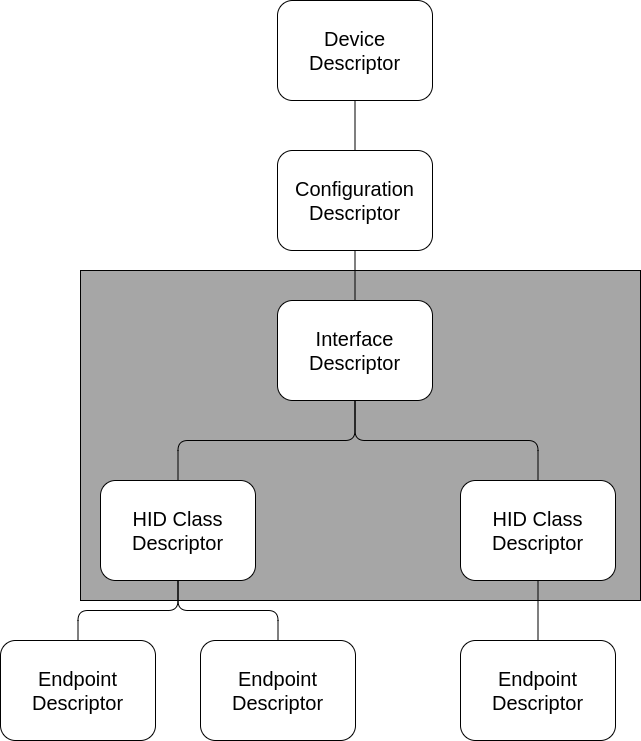
\includegraphics[width=0.5\linewidth]{obrazky-figures/hid_descriptor.png}
    \caption{Layout of descriptors for a composite device that consists of two HIDs.}
    \label{fig:hid_compose}
\end{figure}

\begin{lstlisting}[caption={Example of HID class descriptor in C language},
                   label={lst:hid_example},
                   language=c]
// HID class descriptor
uint8_t desc_hid[] = {
    0x09,                   // bLength
    0x21,                   // bDescriptorType   (HID class)
    WORD_TO_BYTES(0x0100),  // bcdHID
    0x00,                   // bCountryCode      (No localization)
    0x01,                   // bNumDescriptors   (Only reports)
    0x22,                   // bDescriptorType   (REPORT)
    0x40,                   // wDescriptorLength (64 bytes)
};
\end{lstlisting}
\begin{table}[ht]
    \centering
    \begin{tabular}{|l|l|p{0.6\linewidth}|} \hline
         \textbf{Field}     &  \thead{\textbf{Size} \\ \textbf{in bytes}} & \textbf{Description} \\ \hline
         bLength            & 1 & Descriptor size. \\ \hline
         bDescriptorType    & 1 & The constant for HID descriptor type: 0x21. \\ \hline
         bcdHID             & 2 & HID specification release number. \\ \hline
         bCountryCode       & 1 & Country identification number used for localized hardware. \\ \hline
         bNumDescriptors    & 1 & Number of subordinate report and physical descriptors. \\ \hline
         bDescriptorType    & 1 & Type of a class-specific descriptor that follows (0x22 for reports). \\ \hline
         wDescriptorLength  & 2 & The length of the descriptor selected above. \\ \hline
         bDescriptorType    & 1 & \emph{Optional}. Type of a class-specific descriptor that follows (0x23 for physical). \\ \hline
         wDescriptorLength  & 2 & \emph{Optional}. The length of the descriptor selected above. \\ \hline
    \end{tabular}
    \caption{HID class descriptor structure}
    \label{tab:hid_descriptor}
\end{table}

\newpage
\subsection*{Reports}
\label{reports}
As discussed in \autoref{hid}, reports are structures through which the host can send and receive data from the device. The format is very flexible meaning the device can send any type of data. The only limitation is that reports have a fixed size that is defined by a report descriptor.

\textbf{Report descriptor}, like other descriptors, is a structure that specifies the format of the report. It's a class-specific descriptor. If we look at \autoref{fig:hid_compose}, the compose device consists of two HID classes so we have to implement two separate report descriptors for each of them.

The report content format is specified by a list of \emph{items}. Each item is divided into two parts: the first byte identifies the item and the second set of bytes contains data. An example of a keyboard report descriptor that defines an Input report can be found below in \autoref{lst:report_example}.
\begin{lstlisting}[caption={Example of report descriptor in C language},
                   label={lst:report_example},
                   language=c]
uint8_t report_desc[] = {
    0x05, 0x01, // Usage Page (Generic Desktop)
    0x09, 0x06, // Usage (Keyboard)
    0xA1, 0x01, // Collection (Application)
    0x05, 0x07, // Usage Page(Keyboard Usage Page)
    0x19, 0xE0, // Usage Minimum (0xE0)
    0x29, 0xE7, // Usage Maximum (0xE7)
    0x15, 0x00, // Logical Minimum (0x00)
    0x26, 0x01, // Logical Maximum (0x01)
    0x75, 0x01, // Report Size (0x01)
    0x95, 0x08, // Report Count (0x08)
    0x81, 0x02, // Input (Data, Variable, Absolute)
    0xC0,       // End Collection
};
\end{lstlisting}

We can divide items based on the scope of usage: Main, Global, or Local. Items in the main scope define or group data items within a report descriptor. Items in global scope identify and describe what kind of data to expect in the report, such as maximum and minimum values, size of the report, or the number of items in the report. And local items specify the qualities of the controls and data items in a report.

Main scope defines five items: Input, Output, and Feature data items defining the content of a report. Collection and End Collection starts and ends the group. Input items apply to data that is sent from the device to the host. The host uses IN interrupt or Get\_Report request to request Input reports. Output items apply to data that the host sends to the device. They usually change the internal state of the device. For example, to vibrate a game controller during a fight in a game. The host uses OUT interrupt or Set\_Report request to send an Output report. Feature items apply to data that the host sends to the device. But it's not necessary and they can be used the other way around as well. Feature reports update the internal configuration settings of a device that affect the overall behavior of the device. For example, to turn on and off an LED on the keyboard. The host uses both Get\_Report and Set\_Report requests to send/retrieve Feature reports.

Global scope features twelve items which can be seen in \autoref{tab:global_items}. Usage Page specifies the function that the device performs. The HID Usage Table document lists the defined Usage Pages with their values and names. Usage Page are combined with Usage to identify the type of device. For example, Usage Page of \verb|0x01| and Usage of \verb|0x06| tell the host that the given report descriptor sends a keyboard report. Logical and Physical values define what values can report hold. Physical values are used with Units. Unit tag just specifies the unit of the data (time, mass, current. e. g.). It uses the SI (International System of Units) table. Report Size tells the host how many bits are used to encode the data into the report. Report Count tells how many fields will be sent.

\begin{table}[ht]
    \centering
    \begin{tabular}{|l|p{0.7\linewidth}|} \hline
         \textbf{Global Item Type} & \textbf{Description} \\ \hline
         Usage Page & Specifies the data's usage or function \\ \hline
         Logical Minimum & Smallest value that an item will report \\ \hline
         Logical Maximum & Largest value that an item will report \\ \hline
         Physical Minimum & The logical minimum expressed in physical units \\ \hline
         Physical Maximum & The logical maximum expressed in physical units \\ \hline
         Unit Exponent & Base 10 exponent of units \\ \hline
         Unit & Unit values \\ \hline
         Report Size & Size of an item's field in bits \\ \hline
         Report ID & Prefix that identifies a report \\ \hline
         Report Count & The number of data fields for an item \\ \hline
         Push & Places a copy of the global item state table on the stack \\ \hline
         Pop & Replaces the item state table with the last structure pushed onto the stack \\ \hline
    \end{tabular}
    \caption{List of global items}
    \label{tab:global_items}
\end{table}

Local items specify the qualities of the controls and data items in a report. There are ten types of items: Usage, Usage Minimum/Maximum, Designator Index, Designator Minimum/maximum, String Index, String Minimum/Maximum, and Delimiter.
\chapter{BadUSB}
\label{badusb}

BadUSB is a computer security attack that targets peripherals that use USB interfaces. Unlike the usual USB flash disk attacks where the drivers contain harmful files, BadUSB attacks are immune against antivirus programs since the actual code is stored in an inaccessible section of memory. The notion of the attack is to infect the firmware of the USB device. From keyboards and mice to smartphones, if the firmware is reprogrammable then the device is likely exploitable. In 2014 approximately 50 \% of USB microcontrollers  were pruned to this kind of infection.

\subsection*{First appearance}
BadUSB was first revealed during Black Hat conference in the USA. Three security researchers Karsten Nohl, Jakob Lell, and Sascha Krißler demonstrated a collection of proof-of-concept malicious software that highlights the security weakness of the USB\cite{BlackHat}. They spent months reverse-engineering the thumb drive the firmware that runs the basic communication of the device. Nohl and Lell say they've also tested their attack on the Android handset plugged into the PC. And once a BadUSB-infected device is connected to the computer, it could install corrupted software with the backdoor.

Another type of attack was to hijack the internet traffic. The device changes the computer's DNS settings allowing the attack to redirect the traffic to any server he wants. It can also act as a man-in-the-middle, to spy the internet communication on the victim's computer.

The most horrific discovery was the idea that the infection can be spread amongst devices. Once and the USB device is connected to the infected computer, it can be silently reprogrammed with the user detecting anything.

One year later, in December 2015, a group of researchers from University of Florida, David Jing Tian, Adam Bates, and Kevin Butler, published a paper talking about a defense against BadUSB. They built a new layer on top of Linux USB Stack that enforces permissions based on user expectations of device functionality. The additional defense layer (called \emph{GoodUSB}) acts as a mediator and is activated during the enumeration process. GoodUSB restricts USB devices access to USB drivers based on a policy. According to the team, the defense mechanism slows down the enumeration process by only 5.2 \% (from 7 milliseconds to 9 milliseconds)\cite{goodusb}.

\todo{another types of attacks: USBlock: blocking USB-based Keypress Injection Attacks}

\subsection*{Rubber Ducky and Usage}
\label{rubber_ducky}
Rubber Ducky is one of the BadUSB devices that were demonstrated at the conference. They presented an ordinary USB flask drive that acts like a keyboard. Once connected to the computer the device started typing commands. That can be used to open a command prompt to download and install a malicious software, or (since Rubber Ducky lacks video feedback for the attacker) create a reverse shell.

A reverse shell is a concept of connecting to the remote computer from the inside. For example, if I want to connect from the system A to B I can run a program named \textbf{ssh} (Secure Shell) on A. Reverse shell on the other hand run a shell on the system B that opens a shell on system A. What is the advantage of reverse shell? The fact that it bypasses firewall on system B. With reverse shell the attacker has access to the whole PC of a victim.

In 2021, Hongyi Lu and his team at Southern University of Science and Technology published a paper regarding the upgraded version of the device. They implemented a BadUSB on top of a USB device with Type-C connector and named it \emph{BadUSB-C}. Type-C connector supports higher data transmit rate (10 Gbps) which is needed for video capturing. The team fitted a USB device with a Wifi module that lets them see the victim's screen content and control his device using HID emulator (as seen in \autoref{fig:badusbc_model} taken from the original work)\cite{badusbc}.

\begin{figure}[ht]
    \centering
    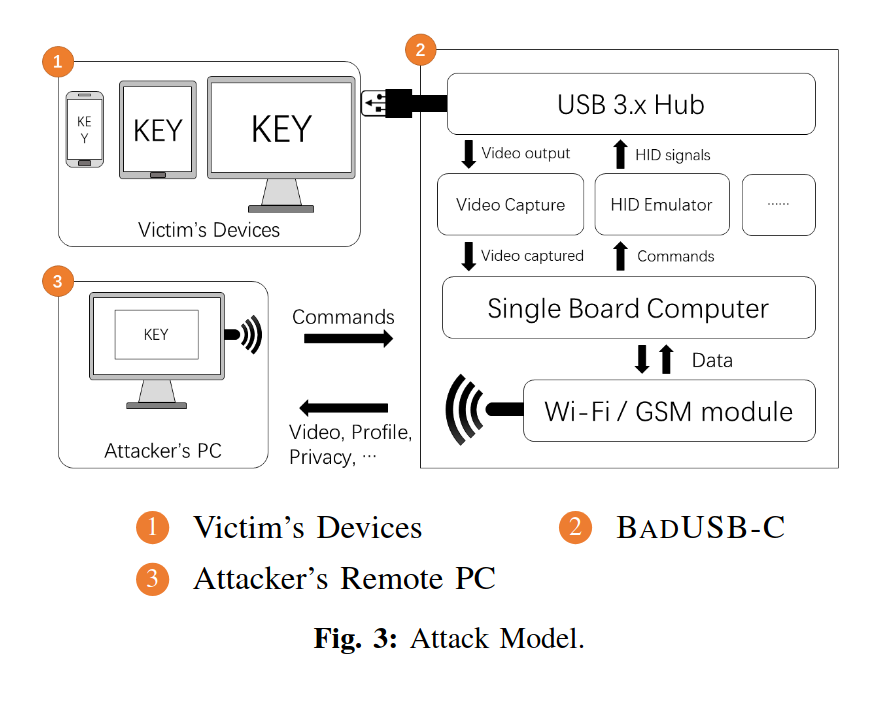
\includegraphics[width=\linewidth]{obrazky-figures/badusbc_attack.png}
    \caption{BadUSB-C's attack model}
    \label{fig:badusbc_model}
\end{figure}

But Rubber Ducky does not have to be seen only as a malicious device. Its ability to perform a script of commands/keystrokes makes it a perfect tool for repetitive tasks. For example, if a user benchmarks computers he can write a script that will configure the computer the same way every time. It's a powerful tool that can greatly help users with everyday tasks but also a dangerous device if used in the wrong way can cause a lot of damage.

% \begin{figure}[ht]
%     \centering
%     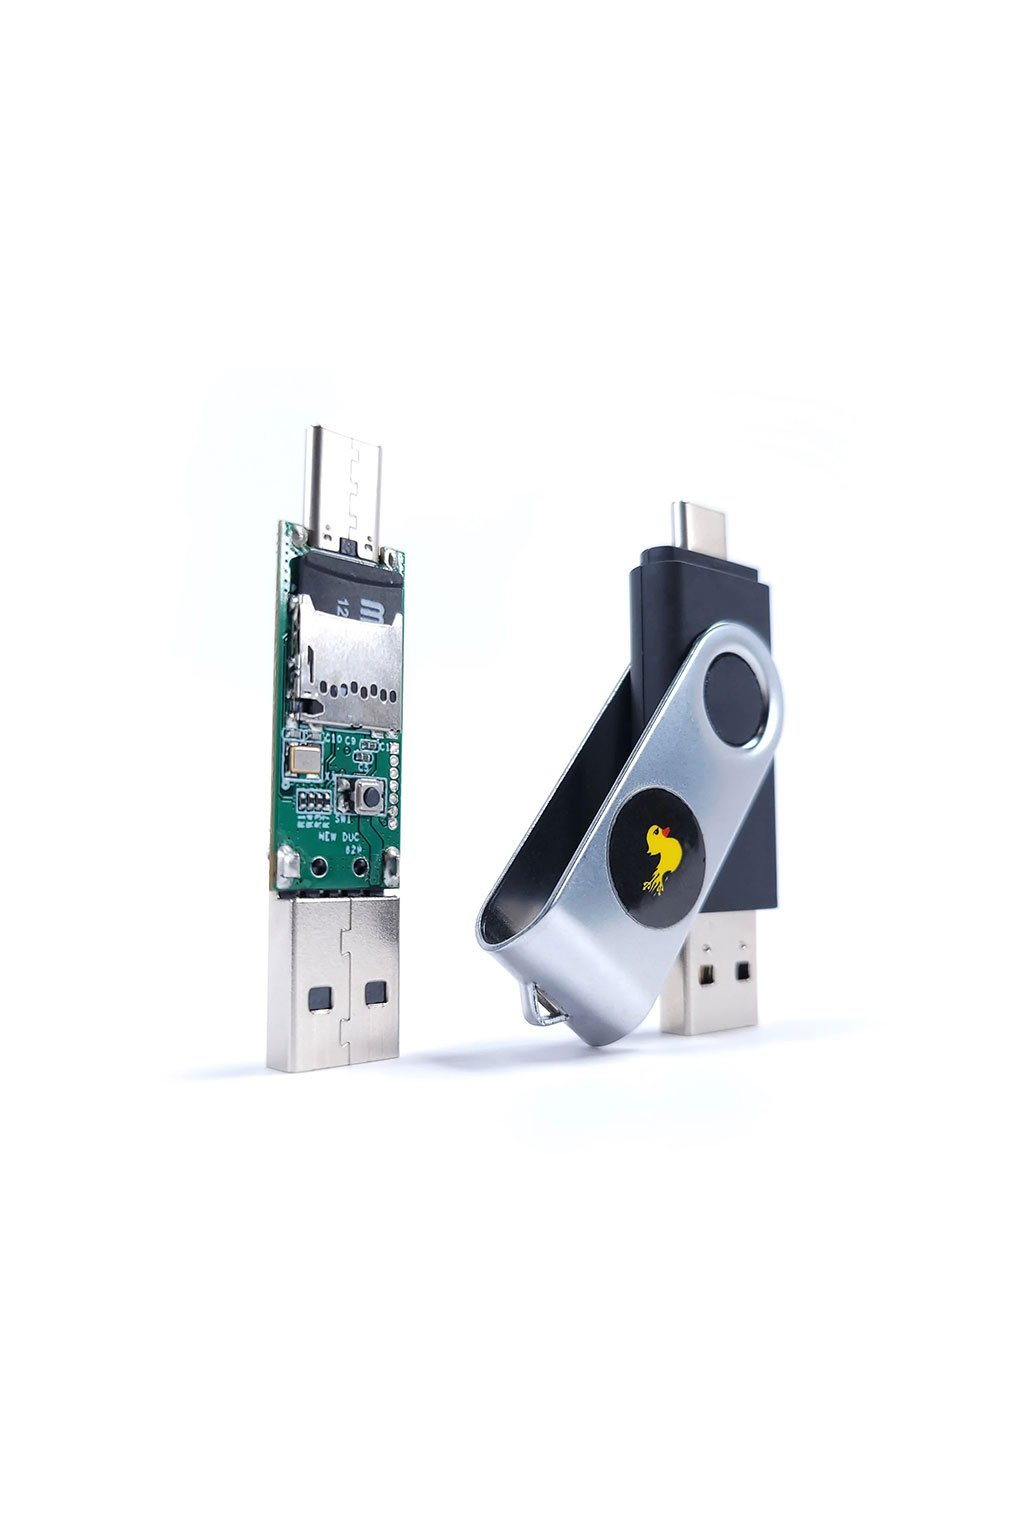
\includegraphics[width=200px]{obrazky-figures/89_usb-rubber-ducky-new.jpg}
%     \caption{Example of Rubber Ducky by Hak5}
%     \label{fig:rubber_ducky}
% \end{figure}
% TODO:

\chapter{Design and Architecture}
\label{designAndArchitecture}
In this section, we analyze the key features of this project. The goal here is to break down the whole problem into manageable parts, identify critical problems and come up with a solution.

Since our device is based on Hak5's Rubber Ducky it must support its main functionality. The device will have the ability to execute a series of keystrokes that are stored within the firmware of the device. The software will provide an easy way to create, generate, and upload these payloads. Together with a keyboard, the device will also include Mass Storage where the user can store a shell basic script or executable file, which he/she can then run it on the host machine.
\todo{add use case diagram}

\section{Base device}
When designing a device capable of a BadUSB attack the first thing to consider is which device we should develop. We wanted a board that is publicly accessible, inexpensive, and easy to work with. After searching the current market we came across \emph{Raspberry Pi Pico} which matches our criteria. \textbf{Raspberry Pi Pico} is a small board with an RP2040 microcontroller chip designed by \emph{Raspberry Pi Foundation}. Its purpose is to encourage people to learn programming and build hardware projects without having to spend lots of money on the hardware itself. We chose a newer version of \emph{Raspberry Pi Pico} model \emph{W} as it also comes with a built-in \emph{CYW43439} wireless chip that supports both Wi-Fi and Bluetooth. That enables us to add a new use case to our project. And with a well-documented SDK\footnote{SDK stands for Software Development Kit} and great support for third-party libraries, this board is a perfect choice for us. \todo{add image of Raspberry Pi Pico W}

\section{Custom Rubber Ducky scripting language}
\label{customLanguage}
First, we need to think of a language that we will use to generate new payloads. The new language has to be intuitive and easy to write in. Since all the device can produce is keystrokes we need to find a to represent each key available on the keyboard. Luckily most (if not all) operating systems come with a keyboard driver preinstalled since it is a commonly used device. For this reason, we don't need to write a driver for our keyboard emulator. \mbox{USB-IF} created a table with a list of supported keys and their IDs\footnote{The usage table can be found here: \url{https://usb.org/sites/default/files/hut1_4.pdf\#chapter.10}}. What that means is that we can build our language based on the IDs. That would be great for the machines as all they have to do is upload it directly to our Rubber Ducky device without any processing (apart from converting the ID values to bytes). But unfortunately, that doesn't meet our criteria for the language to be easy to write it. After all typing \verb|0c 11 17 18 0c 17 0c 19 08|\footnote{If you guessed \textbf{intuitive} then you are a master of ciphers.} feels more as to cipher a message than writing a payload.

Another possible way is to map each ID to a key name. That will make it a lot more human-readable. The only thing left to do is to figure out a way to tell the device to group a set of keystrokes together. Without this feature we would not be capable of producing an upper case \verb|f| since it takes two keys to be pressed at the same time: \textbf{Shift} and \textbf{f} keys.

What I come up with is a language inspired by a VIM key notation\footnote{VIM (which is an acronym to Vi IMproved) is a free open-source text editor. It is known among programmers as a text editor filled with keyboard shortcuts which makes coding and writing much faster and more efficient. Unfortunately, VIM has a steep learning curve making it not beginner-friendly. The official documentation for VIM key notation can be found here: \url{https://vimdoc.sourceforge.net/htmldoc/intro.html\#key-notation}}. The grammar of the language can be represented with a BNF notation seen in \autoref{fig:language_grammar_bnf}.

\begin{figure}[ht]
\begin{verbatim}
<RD-SCRIPT>           ::= <COMMENT><RD-SCRIPT>   |
                          <DELAY><RD-SCRIPT>     |
                          <PRINTABLE><RD-SCRIPT> |
                          <SPECIAL-COMBINATION><RD-SCRIPT> |
                          <EOL>

<COMMENT>             ::= "#" everything after this is ignored

<DELAY>               ::= "<DELAY " <DELAY-VALUE> ">"

<DELAY-VALUE>         ::= positive whole number

<SPECIAL-COMBINATION> ::= "<" <HOLD-VALUE><MODIFIERS><PRINTABLES> ">" |
                          "<" <HOLD-VALUE><MODIFIERS><SPECIAL-KEY> ">"

<HOLD-VALUE>          ::= positive whole number "-" | ""

<MODIFIERS>           ::= <MODIFIER> "-" <MODIFIERS> | ""

<MODIFIER>            ::= modifier short alias

<SPECIAL-KEY>         ::= "\" <SPECIAL-OR-MACRO>

<SPECIAL-OR-MACRO>    ::= special key name | macro name

<PRINTABLES>          ::= <PRINTABLE><PRINTABLES> | ""

<PRINTABLE>           ::= ASCII printable character
\end{verbatim}
\caption{Language grammar in BNF notation}
\label{fig:language_grammar_bnf}
\end{figure}

There are two types of lexical tokens that the language accepts: \emph{printable keys} and \emph{special combinations}.

\textbf{Printable keys} are a group of keys that can produce an ASCII printable character. In total, there are 95 printable characters in the ASCII table ranging from 32, representing a \emph{space} character, to 126, representing a \emph{tilde} character. However, there are only 48 keys that directly produce a printable character. The second half of the keys also require a \emph{shift} modifier (the exception being a spacebar key which doesn't have a shift counterpart). So a string \verb|Hello World!| will produce the following list of keys seen in \autoref{fig:list_of_keys}:

\begin{figure}[ht]
\centering
\begin{varwidth}{\linewidth}
\begin{verbatim}
shift+key_h, key_e, key_l, key_l, key_o, spacebar,
shift+key_w, key_o, key_r, key_l, key_d, shift+key_1
\end{verbatim}
\end{varwidth}
\caption{\emph{Hello world!} converted to key presses.}
\label{fig:list_of_keys}
\end{figure}

One note here: due to the wide variety of different keyboard layouts the official key mapping is only compatible with the \emph{US layout}. What that means is that if the target's machine uses a different keyboard layout than the \emph{US layout} some keys or key combinations will produce a different string than expected. So for example with our machine's keyboard layout set to the Czech QWERTZ, the following set of keystrokes will produce output that the user probably didn't want:
\begin{figure}[ht]
\label{fig:layout_comparison}
\centering
\begin{varwidth}{\linewidth}
\begin{verbatim}
Input:     page_123.cz
US layout: page_123.cz
CZ layout: page%+ěš.cy
\end{verbatim}
\end{varwidth}
\caption{Comparing outputs between cs-CZ and en-US layout given the same input string.}
\end{figure}

A \textbf{Special combination} gives the user more control over the key presses. It extends the functionality by adding features that cannot be executed using only \emph{printable keys}. The format of the \emph{special combination} looks as follows:

\begin{figure}[ht]
\label{fig:format_special}
\centering
\begin{varwidth}{\linewidth}
\verb|"<" [special_combination_content] ">"|
\end{varwidth}
\caption{\emph{Special combination}'s content is wrapped in < and > symbols}
\end{figure}

There are four features that the user can define within the scope:
\begin{itemize}
    \item \emph{waiting time} between the keystrokes,
    \item pressing \emph{non-printable keys},
    \item pressing keys with \emph{modifiers} with an option to set a \emph{holding time},
    \item force multiple \emph{printable key} pressed simultaneously.
\end{itemize}

\textbf{Waiting time} or \textbf{delay} tells the device how long it has to wait before sending the next series of keystrokes to the host. This is very important, without it the payloads would fail most of the time since the device usually needs to wait until a GUI element loads or a file is downloaded. The format of a delay command looks as followed: \verb|<DELAY [delay_in_ms]>|. An example of the usage of the delay command can be seen in \autoref{fig:delay_example}.

\begin{figure}[ht]
\centering
\begin{varwidth}{\linewidth}
\verb|take <DELAY 5000> dave brubeck|
\end{varwidth}
\caption{In this example the USB device will type "take " string, wait 5 seconds, and finish by typing the string " dave brubeck".}
\label{fig:delay_example}
\end{figure}

\textbf{Non-printable keys} are, as the name suggests, keys that don't produce any printable characters \-- in other words all other keys. Of course, there are some notable exceptions. Even though \verb|Keypad_1| or \verb|Keypad_Asterisk| keys all produce a printable character (\verb|'1', '*'| respectively), they are not considered printable keys and to access them the user has to explicitly put them in the \emph{special combination} format in order to execute them. To differentiate non-printable keys from printable keys to former is written together with a \verb|\| prefix. Examples of non-printable keys can be seen in \autoref{fig:non_printable_example}. The parser doesn't distinguish between uppercase and lowercase letters (case-insensitive).

\begin{figure}[ht]
\centering
\begin{varwidth}{\linewidth}
\begin{verbatim}
<\enter><\SPACEBAR><\BackSpace><\arrow_up><\f12><\num1><\volume_up>
\end{verbatim}
\end{varwidth}
\caption{Examples of non-printable key presses in custom Rubber Ducky script language.}
\label{fig:non_printable_example}
\end{figure}

Other additions to \emph{non-printable keys} are supports for \emph{modifier keys} and \emph{holding time}. \textbf{Modifier keys} are special keys that temporarily alter the action of a normal key (printable or non-printable key) when pressed together. There are in total 8 modifier keys:
\begin{itemize}
    \item left and right \verb|Alt|,
    \item left and right \verb|Control|,
    \item left and right \verb|Meta| (also known as Windows, Hyper, Super, or Command key depending on the operating system),
    \item left and right \verb|Shift|.
\end{itemize}
 We have already encountered a modifier key when discussing printable keys. When we press \verb|Shift| key together with \verb|Key_s| the \emph{shift} key changes the action of the \emph{s} key to output upper case \emph{S} instead of lowercase \emph{s} it would normally output. We can also associate modifier keys with keyboard shortcuts, the most famous one being \verb|alt+f4| to close an active window on Windows or \verb|ctrl+s| to save the content of a file. Modifier keys usually don't produce any action when pressed alone (Meta key notably being an exception) so they are handled differently when sending keystrokes to the host's machine. In the \emph{special combination} format modifier keys are placed before normal keys as seen in \autoref{fig:language_grammar_bnf}. Each modifier is identified by the location of the key followed by its starting letter \-- \verb|'la'| for \verb|LeftAlt|, \verb|'rs'| for \verb|RightShift|, and so on. If the user doesn't specify which one of the keys is meant, the left one will be chosen implicitly \-- \verb|'m'| will trigger \verb|LeftMeta|, \verb|'c'| will trigger \verb|LeftControl|, and so on. Each key is then separated with a \verb|-| separator.

\textbf{Holding time}, as the name suggests, defines how long a group of keys is meant to be pressed before releasing, measured in milliseconds. The hold delay value is expected to be at the start of the \emph{special combination}. This field is not required to be filled and the implicit value is set to 0.

The last thing the \emph{special combination} scope supports is to force multiple \emph{printable keys} to be pressed at the same time. That is especially useful when the user wants to execute a keyboard shortcut that consists of two or more normal keys. As an example, we can use Visual Studio Code's\footnote{Visual Studio Code is a popular graphical text editor developed by Microsoft that supports extensions: \url{https://code.visualstudio.com/}} keyboard shortcut for closing all files in the editor: \verb|Ctrl+k Ctrl+w|. The language's equivalent of the given keystrokes is \verb|<c-kw>|.

There are some letters that would not work in this format, \verb|<| and \verb|>| being the case. For that, I created a group of \emph{macro keys}. A \textbf{Macro key} is an alias to an existing key. It can be an alias to either the normal key or modifier key and is treated the same way as a \emph{non-printable key} \-- it starts with an escape backslash character followed by the name of the macro. So we can use \verb|<\gt>| and \verb|<\lt>| in to produce \verb|<| and \verb|>| respectively.

The last feature of the language is the ability to write \emph{comments}. The comment grammar is inspired by scripting programming languages such as Bash or Python. It starts with \verb|#| symbol and the characters that follows this symbol are all ignored by the parser until the end of the line. There are no multi-line comments support. If the user wants to type a \verb|#| symbol he/she needs to put it into the \emph{special combination} scope.

The following \autoref{lst:example_payload} shows an example payload written showcasing all the grammar syntax of the language.
\begin{lstlisting}[caption={Example payload in custom language.},
                   label={lst:example_payload}]
# ============================================================
# This is a single line comment

# let's open a terminal on Ubuntu using its keyboard shortcut
# and wait 500ms for it to open
<c-a-t><DELAY 500>

# ... now run a command
echo "hello world!"

# ... it doesn't work :( oh wait we must run it first!
<\enter>    # yay it outputs hello world!

# lets run some calculation in python now
python -c "a = 2<\enter><#> a = 4<\enter>print(a <\lt> 3)"<\enter>

# the commands from above should produce something like this
#     $ python -c "a = 2
#     # a = 4
#     print(a < 3)"

# now lets find the oldest command run on the machine!
# hopefully 10 seconds will be enough
<10000-\arrow_up><\enter>

# that is the end of our Linux terminal scripting 101 tutorial
# ============================================================
\end{lstlisting}

\section{Communication protocol}
\label{communicationProtocol}
Since our development board supports WiFi we made a decision to create a communication protocol and a network application based on it. Let our Rubber Ducky device be \emph{server} and our network application be \emph{client}. We need to define use cases for each side. This is a list of requests that we want the client to support:
\begin{itemize}
    \item Notify the device (server) that the client will send a new payload.
    \item Send to the device a new series of keystrokes.
    \item Remove the last sent set of keystrokes.
    \item Retrieve keystrokes from the device.
    \item Start the stored payload execution.
\end{itemize}

The server, on the other hand, will have only two types of responses: an \textbf{OK} response which signalizes that the request was successfully processed and an \textbf{ERR} response with an error message when something unexpected happened while processing the request.

What we came up with is a communication protocol on L7 application layer\footnote{More about Internet Network's ISO/OSI model here: \url{https://www.ietf.org/rfc/rfc1122.txt}} with a diagram shown in \autoref{fig:communication_protocol_packet_format}, \autoref{fig:communication_protocol_request}, and \autoref{fig:communication_protocol_response}. We wanted to simplify the packet's structure as much as possible. The packet header is 4 bytes long with the rest of the packet being filled with the packet's content (payload data).

\begin{figure}[ht]
\centering
\begin{varwidth}{\linewidth}
\begin{verbatim}
                  Packet format
                  =============

      0           1           2           3
+-----------+-----------+-----------+-----------+
|  OP CODE  | RESERVED  |    PAYLOAD LENGTH     |
+--+--+--+--+--+--+--+--+--+--+--+--+--+--+--+--+
|                PAYLOAD DATA                   |
/                                               /
+--+--+--+--+--+--+--+--+--+--+--+--+--+--+--+--+
\end{verbatim}
\end{varwidth}
\caption{Communication protocol's packet format used in the project.}
\label{fig:communication_protocol_packet_format}
\end{figure}

The first being of the header contains an \textbf{operational code}. It tells the server what kind of action we are requesting as well as informs the client about the operation's result. All operational codes are analyzed later in this section. The second byte in the header is \textbf{reserved} due to structure padding in C programming language. \todo{reference to a book}
Last two bytes in the header store \textbf{the size of the payload data}. Two bytes here will give us values ranging from 0 to 65 535 which should be plenty enough to carry the payload.

Next, we can analyze the request packet structure. Our project supports 9 \emph{operational codes} as shown in \autoref{fig:communication_protocol_request}. We can divide them into 4 groups:

\begin{enumerate}
    \item work with the USB device's (server's) inner read-write mode,
    \item update device payload,
    \item analyze the payload stored on the device,
    \item run the payload.
\end{enumerate}

\begin{figure}[ht]
\centering
\begin{varwidth}{\linewidth}
\begin{small}
\begin{verbatim}
                             Request
                             =======
Operation codes and their values:
+----+-------------+---------+--------------+--------------------------+
| op |   opcode    | payload |   expected   |       description        |
|    |    name     |  size   |     value    |                          |
+----+-------------+---------+--------------+--------------------------+
| 01 |     SET     |   01    |    00/01     |   Enable/disable device  |
|    |  EDITABLE   |         |              |      read-write mode     |
+----+-------------+---------+--------------+--------------------------+
| 02 |     GET     |   00    |      --      |      Check device's      |
|    |  EDITABLE   |         |              |  read-write mode status  |
+----+-------------+---------+--------------+--------------------------+
| 03 | CLEAR DATA  |   00    |      --      |      Clear device's      | *
|    |             |         |              |     current payload      |
+----+-------------+---------+--------------+--------------------------+
| 04 |  PUSH DATA  |   0d    | key sequence | Send a new key sequence  | *
+----+-------------+---------+--------------+--------------------------+
| 05 |  POP DATA   |   00    |      --      | Remove last key sequence | *
+----+-------------+---------+--------------+--------------------------+
| 06 |  GET DEBUG  |   00    |      --      | Retrieve a key sequence  |
|    |   CURSOR    |         |              |       at the debug       |
|    |             |         |              |     cursor's position    |
+----+-------------+---------+--------------+--------------------------+
| 07 | INC DEBUG   |   00    |      --      | Move debug cursor to the |
|    |   CURSOR    |         |              |    next key sequence     |
+----+-------------+---------+--------------+--------------------------+
| 08 | RESET DEBUG |   00    |      --      |   Reset debug cursor's   |
|    |   CURSOR    |         |              |         position         |
+----+-------------+---------+--------------+--------------------------+
| 09 |     RUN     |   00    |      --      | Tell the device to start | **
|    |  SEQUENCES  |         |              |  executing the payload   |
+----+-------------+---------+--------------+--------------------------+

*  - device must be set to read-write mode to run this command
** - device must be set to read-only mode to run this command
\end{verbatim}
\end{small}
\end{varwidth}
\caption{Set of request's operational codes, their payload, and description.}
\label{fig:communication_protocol_request}
\end{figure}

The first two operational codes fall under the first group. Their purpose is to change or check whether the device is currently in read-write mode. There are other actions that depend on it. \verb|SET_EDITABLE| (0x01) sends a single-byte payload of 0x00, which will set device to \emph{read-only} mode, or 0x01, which will switch the device to \emph{read-write} mode. \verb|GET_EDITABLE| (0x02) retrieves the current mode present on the device.

The second group's purpose is to alter the payload stored on the device. It is required for the device to be in \emph{read-write} mode. Otherwise, the device will respond with an error message and the action will be ignored. \verb|CLEAR_DATA| (0x03) action removes the current payload from the device. \verb|PUSH_DATA| (0x04) uploads a new \emph{key sequence} to the device. The payload should contain the \emph{key sequence} data already reshaped to the desired format expected by the device\footnote{The expected format can be seen in \autoref{fig:key_sequence_format}. It is a 13 bytes long structure where \emph{waiting delay} occupies the first 4 bytes, followed by a 1 bitmap of \emph{modifiers} (\texttt{MDFR}), a reserved byte, 6 keyboards key IDs (see \autoref{customLanguage}), and a \texttt{LAST} byte, which indicates that this key sequence will be the last one in the series.}. \verb|POP_DATA| (0x05) removes the last inserted key sequence. Users can retrieve it from the server response payload.

\begin{figure}[ht]
\centering
\begin{varwidth}{\linewidth}
\begin{verbatim}
    0     1      2      3      4      5      6      7
+------+------+------+------+------+------+------+------+
|            DELAY          | MDFR | RESV | KEY1 | KEY2 |
+------+------+------+------+------+------+------+------+
| KEY3 | KEY4 | KEY5 | KEY6 | LAST |
+------+------+------+------+------+
\end{verbatim}
\end{varwidth}
\caption{Key sequence format}
\label{fig:key_sequence_format}
\end{figure}

The third group contains actions that serve as a debug tool for the user. The debug cursor always starts at the beginning of the series. A request with \verb|GET_DEBUG_CURSOR| (0x06) will retrieve a \emph{key sequence} which is currently under the cursor. To get the next key sequence the user needs to send a \verb|INC_DEBUG_CURSOR| (0x07) which moves the cursor to the next one (if it is available). Finally, the \verb|RESET_DEBUG_CURSOR| (0x08) request moves it back to the beginning.

The last operation on the list is a \verb|RUN_SEQUENCES| (0x09). As the name suggests, this request will start executing the payload on the device. The only requirement here is that the device must be in \emph{read-only} mode.

Now, we can analyze the last two operation codes which we can see in \autoref{fig:communication_protocol_response}. They are used by the server as a form of response to requests. \verb|OK| response is generated when the request is successfully generated. It can carry some data depending on the received request (for example \emph{key sequence} data as an answer to \verb|POP_DATA|, or device mode when received \verb|GET_EDITABLE|). The other type of response is \verb|ERR| which is generated when an error occurred during the request processing. This response will always carry the error message in its payload.

\begin{figure}[ht]
\centering
\begin{varwidth}{\linewidth}
\begin{verbatim}
                           Response
                           ========

+----+------+-------------+---------------------------+-----------+
| op | name | payload_len |       description         |  payload  |
+----+------+-------------+---------------------------+-----------+
| 0a | OK   |   varies    | Request was successfully  | data from |
|    |      |             |         processed         |   server  |
+----+------+-------------+---------------------------+-----------+
| 0b | ERR  |   varies    | Request was not correctly |   error   |
|    |      |             |         processed         |  message  |
+----+------+-------------+---------------------------+-----------+
\end{verbatim}
\end{varwidth}
\caption{Set of responses, their content, and description.}
\label{fig:communication_protocol_response}
\end{figure}

Let's end this section with a data flow diagram showcasing a possible communication between the \emph{server} (device) and the \emph{client} (user) shown below in \autoref{fig:dataflow_example}:

\begin{figure}
    \centering
    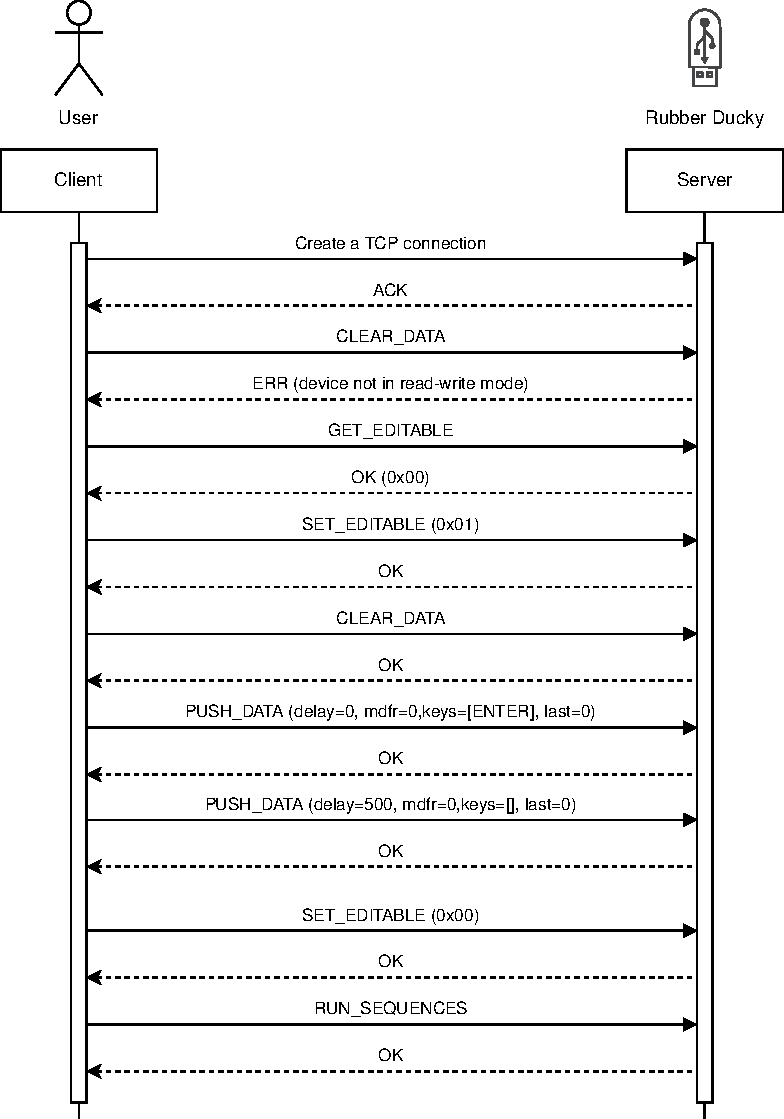
\includegraphics{obrazky-figures/dataflow.pdf}
    \caption{Example of the communication between the client and the server. In this example, the user sends two key sequences to the device: \texttt{<\textbackslash{}enter><DELAY 500>}. We can also see the user making a mistake at the beginning of the communication by sending a \texttt{CLEAR\_DATA} request when the device is still in \emph{read-only mode}.}
    \label{fig:dataflow_example}
\end{figure}

\chapter{Implementation of Rubber Ducky-like device}
\label{implementation}
The purpose of this section is the familiarize the user with the actual structure of this project. The goal here is to show the reader how each part of the software is implemented. The design from \autoref{designAndArchitecture} will serve as our main source and all implemented parts of this project will be based on it.

The first half of the chapter is dedicated to the Rubber Ducky software which I wrote using C programming language and all the source codes are present in \verb|rubber_ducky| directory, and the second half of the chapter deals with the Rubber Ducky scripting language and the client application for which I used Python and the code is located in \verb|rd_client| directory.

\section{Used third-party libraries}
This project was developed using four open-source an SDK and libraries:
\begin{description}
    \item [pico-sdk] The Raspberry Pi Pico SDK (henceforth the SDK) provides the headers, libraries and build system necessary to write programs for the RP2040-based devices such as the Raspberry Pi Pico in C, C++, or assembly language.\footnote{\url{https://github.com/raspberrypi/pico-sdk}}
    \item [cyw43-driver] An open-source library which implements a driver for CYW43xx WiFi/BT SoC.\footnote{\url{https://github.com/georgerobotics/cyw43-driver}}
    \item [TinyUSB] TinyUSB is an open-source cross-platform USB Host/Device stack for embedded systems, designed to be memory-safe with no dynamic allocation and thread-safe with all interrupt events deferred and then handled in the non-ISR task function.\footnote{\url{https://github.com/hathach/tinyusb}}
    \item [lwIP] lwIP library is a small independent implementation of the TCP/IP protocol suite. The focus of the lwIP TCP/IP implementation is to reduce the RAM usage while still having a full-scale TCP.\footnote{\url{https://github.com/lwip-tcpip/lwip}}
\end{description}

\section{Rubber Ducky device}
This section gives an overview on how the software on the Raspberry Pi Pico was implemented. The class diagram can be seen in \autoref{fig:rubber_ducky_module}.

\begin{figure}[ht]
    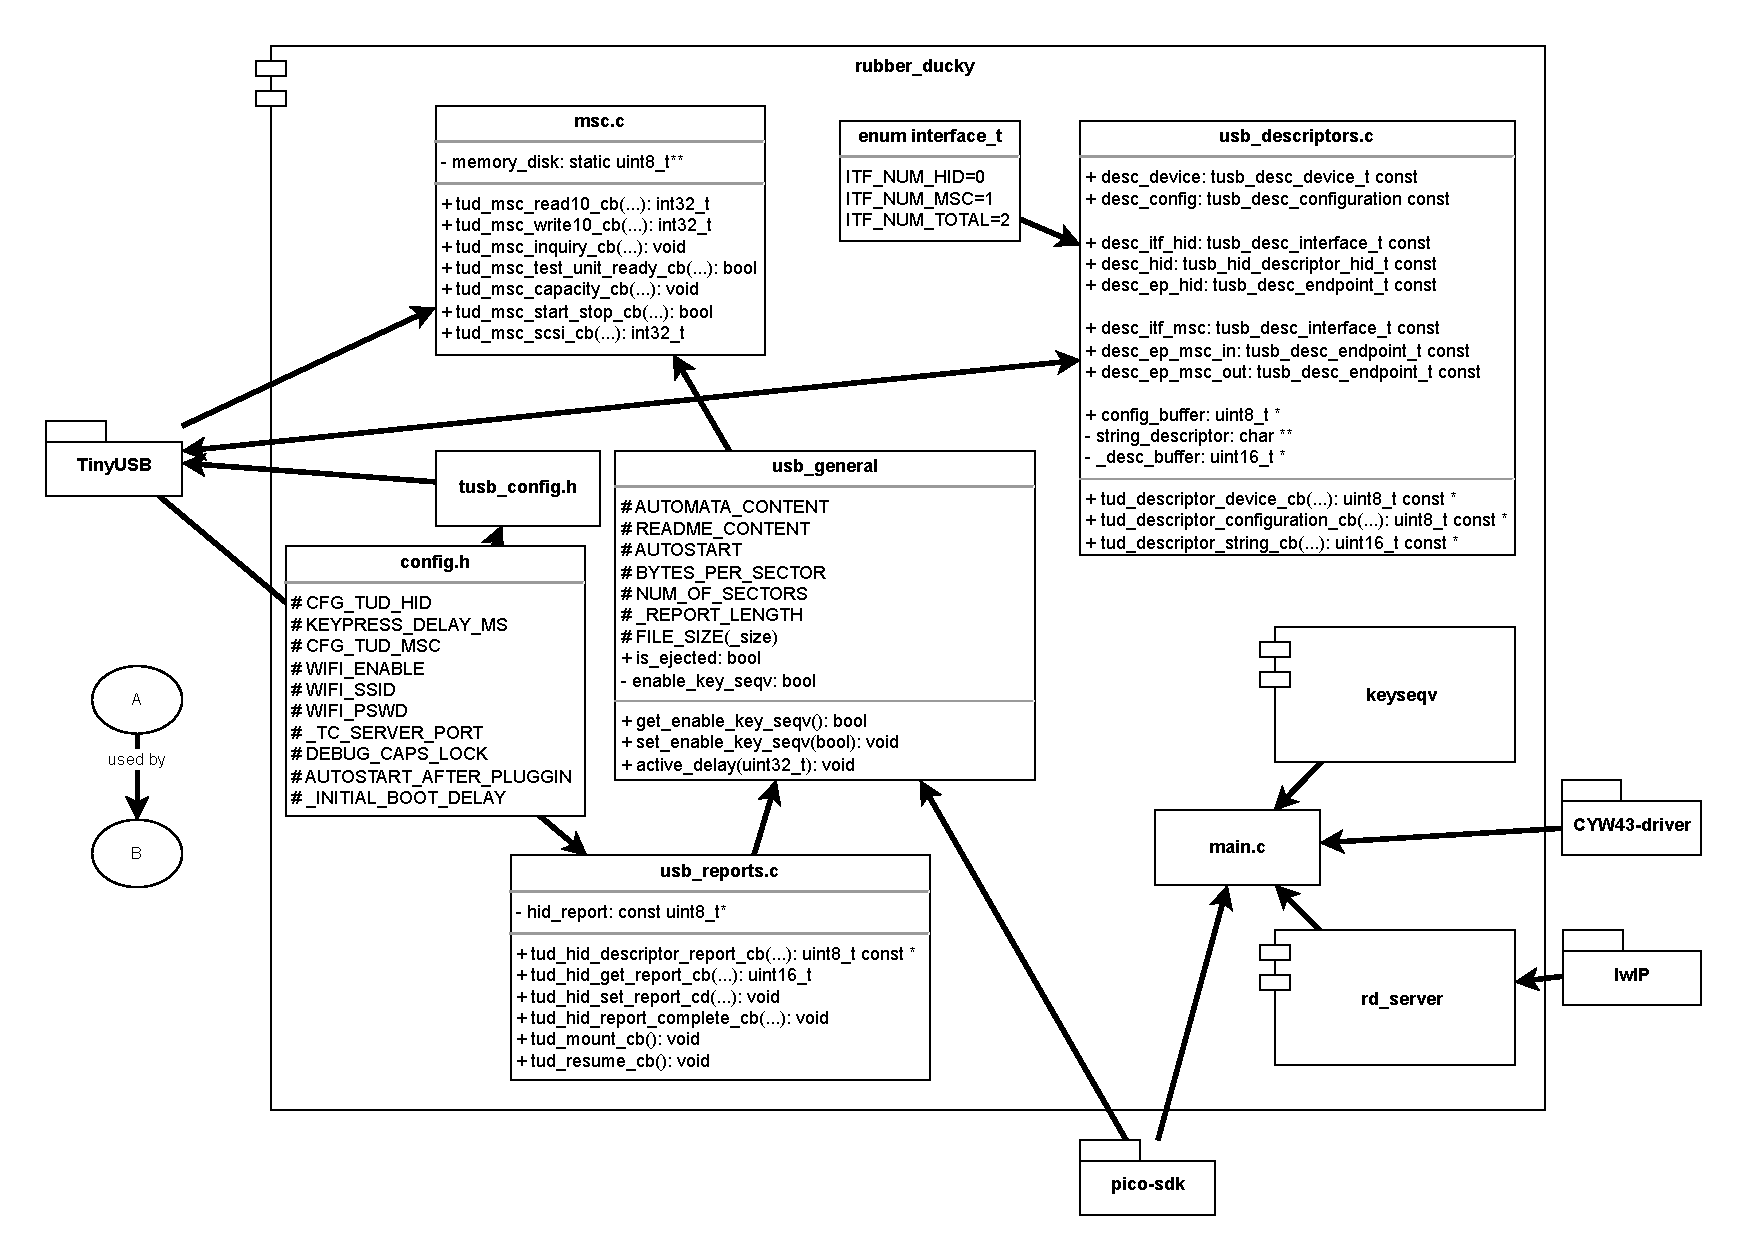
\includegraphics[width=\linewidth]{./obrazky-figures/rubber_ducky_module.pdf}
    \caption{RubberDucky module UML class diagram.}
    \label{fig:rubber_ducky_module}
\end{figure}

\subsection{USB configuration}
In the first part, I needed to configure the USB device to make it ready for the enumeration process. TinyUSB library requires \verb|tusb_config.h| header file, which defines configuration macros, such as \verb|CFG_TUD_ENABLED| to set the device as a "device" and not as a "host", or \verb|CFG_TUD_HID| which defines how many HID configurations will the device have, and more. Part of the configuration was moved to \verb|config.h| header file. This file contains macros that the user can freely edit. \verb|config.h| is then imported to \verb|tusb_config.h|.

Next, I had to configure the Raspberry Pi Pico board to behave like a keyboard and mass storage simultaneously. As previously mentioned in \autoref{usb}, the host identifies the USB device's identity by retrieving its descriptor and configurations. TinyUSB defines 3 callback functions for that:
\begin{enumerate}
    \item \verb|tud_descriptor_device_cb| -- A callback function which the host uses to retrieve \emph{device descriptor}.
    \item \verb|tud_descriptor_configuration_cb| -- A callback function which the host uses to retrieve every \emph{configuration descriptors} present on the device. It also includes \emph{interface descriptors}, \emph{device class descriptors} (if exists), and \emph{endpoint descriptors}.
    \item \verb|tud_descriptor_string_cb| -- A callback function which the host uses to retrieve \emph{string descriptors} based on the index.
\end{enumerate}

\verb|usb_descriptors.c| defines all three callback functions. I created instances of descriptors with the structures provided by the library and wrote each callback function's logic to return a pointer to those instances (see an example in \autoref{lst:descriptor_cb}).

\begin{lstlisting}[caption={Definition of the \emph{device descriptor} and its callback function used in \texttt{usb\_descriptors.c}.},
                   label={lst:descriptor_cb},
                   language=c]
// device descriptor
tusb_desc_device_t const desc_device = {
    .bLength            = sizeof(tusb_desc_device_t),
    .bDescriptorType    = TUSB_DESC_DEVICE,     // DEVICE constant
    .bcdUSB             = 0x0110,   // USB1.1
    .bDeviceClass       = 0x00,
    .bDeviceSubClass    = 0x00,
    .bDeviceProtocol    = 0x00,
    .bMaxPacketSize0    = CFG_TUD_ENDPOINT0_SIZE,

    // list of vendors found here: http://www.linux-usb.org/usb.ids
    .idVendor           = 0xD0D0,   // vendor's id (must be unique)
    .idProduct          = 0xCAFE,   // product id (must be unique with vendor)
    .bcdDevice          = 0x0100,   // version

    .iManufacturer      = 0x01,     // string index of manufacture name
    .iProduct           = 0x02,     // string index of product name
    .iSerialNumber      = 0x00,

    .bNumConfigurations = 0x01 // number of configuration
};

// ...

uint8_t const * tud_descriptor_device_cb() {
    return (uint8_t const *) &desc_device;
}
\end{lstlisting}

\subsection{The keyboard}
Since a keyboard is categorized as a \emph{human interface device} I had to define its report structure. That is defined in \verb|usb_reports.c| file. A keyboard report consists of three parts:
\begin{enumerate}
    \item a modifier bitmap, which is sent to the host,
    \item an LED bitmap, which is received from the host,
    \item and up to 6 keycodes, which are sent to the host.
\end{enumerate}
I created a huge byte array named \verb|hid_report|, which I loaded with the report byte codes. Then I defined the required HID callback functions. To ease myself during the testing of the device I added a debugging feature. If the user turns the Caps Lock LED on and off, the device will start executing the payload once again. The logic here is very simple and can be seen in \autoref{lst:usb_debug}. In order for this to work, the user needs to set a \verb|DEBUG_CAPS_LOCK| macro to 1 in the \verb|config.h| header file.

\todo{new code here}
\begin{lstlisting}[caption={A snippet of code which implements the payload re-execution.},
                   label={lst:usb_debug},
                   language=c]
void tud_hid_set_report_cb(uint8_t instance, uint8_t report_id,
                           hid_report_type_t report_type,
                           uint8_t const* buffer, uint16_t bufsize) {
    // ignore this request
    (void) instance;
    (void) report_id;
    (void) report_type;
    (void) buffer;
    (void) bufsize;
#if DEBUG_CAPS_LOCK
    if (buffer == NULL || bufsize <= 0)
        return;
    if (report_type != HID_REPORT_TYPE_OUTPUT)
        return;

    // reset key sequence when caps lock is turned off
    if (!(buffer[0] & KEYBOARD_LED_CAPSLOCK)) {
        key_seqv_reset_index_counter(false);
        if (!get_enable_key_seqv()) {
            set_enable_key_seqv(true);
        }
    }
#endif
}
\end{lstlisting}

\subsection{The mass storage}
Mass storage configuration is located, surprisingly, in \verb|msc.c| file. TinyUSB library requires 6 callback functions to be defined in order for the mass storage device to run:
\begin{itemize}
    \item \verb|tud_msc_read10_cb| -- Returns a content of a memory sector given an address of the sector.
    \item \verb|tud_msc_write10_cb| -- Updates a content of a memory sector given an address of the sector.
    \item \verb|tud_msc_inquiry_cb| -- Returns Vendor ID, Product ID, and Product revision number of the device.
    \item \verb|tud_msc_test_unit_ready_cb| -- Returns true allowing the host to read and write on the device.
    \item \verb|tud_msc_capacity_cb| -- Determines a disk size.
    \item \verb|tud_msc_scsi_cb| -- Defines the logic of other SCSI commands.
\end{itemize}
Unfortunately, due to Raspberry Pi Pico's lack of onboard nonvolatile memory, I had to write a static file system from scratch. I chose a \textbf{FAT12} file system since it is one of the simplest file systems out there and for the proof of concept a sufficient one. The whole content of the file system is stored in the \verb|memory_disk| array which emulates a physical disk. It is represented as a two-dimensional array with the first dimension emulating an array of \emph{sectors} and the second dimension being the \emph{sector}\footnote{A sector is an elementary storage unit. It is the smallest number of bytes that the host can retrieve from the disk.} itself. The first sector contains a \textbf{boot table}, the second one is a \textbf{FAT table}, the third one is a \textbf{root directory}, and the rest of the disk is filled with file contents. Each part of the file system is described in \cite{fatFS}.

\subsection{The payload}
\label{thePayload}
The payload and its API are managed in \verb|keyseqv| directory. Each key sequence is represented by a \verb|key_seqv_t| structure which can be seen in \autoref{fig:keyseqv_module}. It contains three members: a \textbf{delay} that will be applied after sending the report to the host, the \textbf{report} with key presses itself, and a \textbf{last item} flag which tells the device to not send any report after this one. The whole payload is then stored in \verb|key_seqvs| array and defined in \verb|key_seqv_script.c| source file. This file can be generated by \verb|rd_client| script.
\begin{figure}[ht]
    \centering
    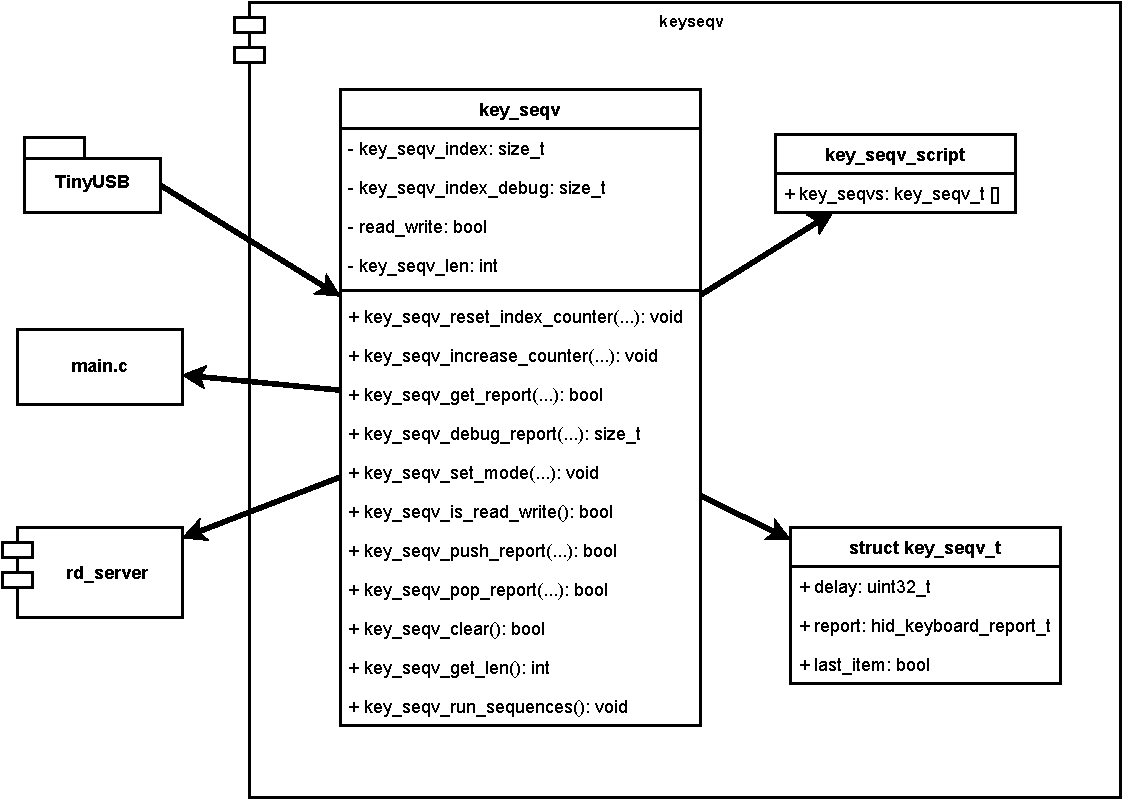
\includegraphics[width=0.8\linewidth]{./obrazky-figures/keyseqv_module.pdf}
    \caption{Keqseqv module UML class diagram.}
    \label{fig:keyseqv_module}
\end{figure}

Lastly, the \verb|key_seqv.c| source file defines all the functions that operate directly with the \verb|key_seqv_t| structure. That includes functions that update the payload content through the server's API (more in the next section) and those that are used for executing the payload. The two most important functions here are named \verb|key_seqv_increase_counter| \linebreak which moves the cursor index to the next item (key sequence) in the array, and \linebreak\verb|key_seqv_get_report| which retrieves the current report from the array.

Putting these last two functions together we can see the pseudocode of the core algorithm of executing the payload in \autoref{alg:payload_exec} shown below:

\begin{algorithm}
\caption{Payload execution algorithm}
\label{alg:payload_exec}
\KwIn{\texttt{cursor}, \texttt{key\_seqvs}}
\BlankLine
device initialization\;
\While{true}{
    process USB device tasks\;
    retrieve an \texttt{item} from \texttt{key\_seqvs} at \texttt{cursor}'s position\;
    \eIf{execution not enabled or \texttt{item} is empty}{
        \texttt{delay} = 0\;
        \texttt{report} = empty report\;
        send a \texttt{report} to host\;
    }{
        \texttt{delay} = \texttt{item}.delay\;
        \texttt{report} = \texttt{item}.report\;
        send a \texttt{report} to host\;
        \If{\texttt{report} sent successfully}{
            increase the \texttt{cursor} position in \texttt{key\_seqvs}\;
            wait \texttt{delay} before executing next key sequence\;
        }
    }
}
\end{algorithm}

\section{WiFi Access Point and TCP Server}
\begin{figure}[ht]
    \centering
    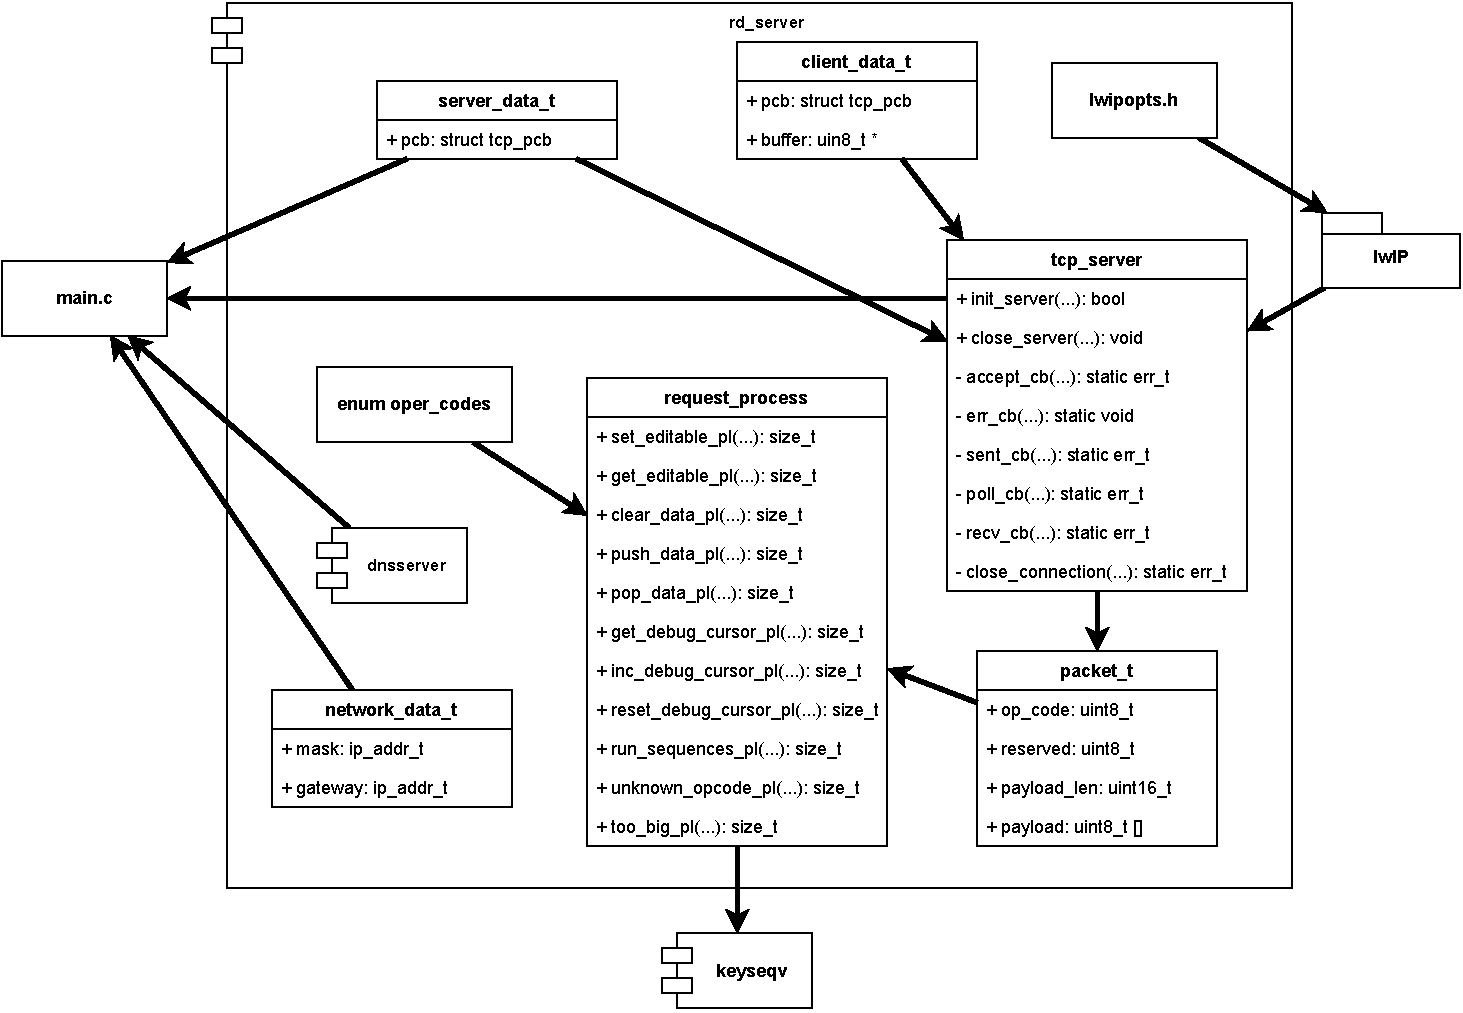
\includegraphics[width=\linewidth]{./obrazky-figures/rd_server_module.pdf}
    \caption{RD Server module UML class diagram.}
    \label{fig:rd_server_module}
\end{figure}
To run a server we need 2 things: a port and an IP address of the server. But first, the Raspberry Pi Pico device needs to be connected to the network. There are two ways to achieve this: the device can either connect to the local WiFi once it is powered up, or it can create an access point and let the client connect to its WiFi network. I chose to implement the latter one. The advantage of having the device being an access point is that I know the IP address of the server \--- it is the IP address of the network's gateway. The disadvantage is that I need to implement a DHCP server\footnote{DHCP (Dynamic Host Configuration Protocol) is a network management protocol used to dynamically assign an IP address to any device, or node, on a network so it can communicate using IP (source: \url{https://www.techtarget.com/searchnetworking/definition/DHCP})} in order to have a functional network.

In order for the device to act as an access point the user needs to set \verb|WIFI_ENABLE| macro, network's SSID (or simply a name), and password, all in \verb|config.h| header file. Once done, Raspberry's software will call \verb|cyw43_arch_enable_ap_mode| during the initialization phase.

After the access point is running, the TCP servers for DHCP and our application are initialized. They are all defined in \verb|rd_server| directory seen in \autoref{fig:rd_server_module}. The source codes for the DHCP server are taken over from Raspberry Pi Pico's example page\footnote{DHCP server source codes: \url{https://github.com/raspberrypi/pico-examples/tree/master/pico_w/wifi/access_point}}. We initialize the DHCP server by providing the network's gateway and mask (see \autoref{lst:dhcp_config}). There is no DNS server in this network since we only want to create communication between the USB device and a client's application and that will be happening in the isolated private network.

\lstset{
    caption={A basic network configuration used in the project. In this case, the IP address of the network is \textbf{192.168.4.0/30}.},
    label={lst:dhcp_config},
    language=c,
}
\begin{lstlisting}
int main() {
    // ...

    // define network's IP range
    struct network_data_t nd;
    IP4_ADDR(ip_2_ip4(&(nd.gateway)), 192, 168, 4, 1);
    IP4_ADDR(ip_2_ip4(&(nd.mask)), 255, 255, 255, 252);

    dhcp_server_t dhcp_server;
    dhcp_server_init(&dhcp_server, &(nd.gateway), &(nd.mask));

    // ...
}
\end{lstlisting}

There are two source files that deal with our server application: \verb|tcp_server| and \verb|request_process|. The former defines a TCP socket server using lwIP library, and the latter defines functions that process requests. The server waits for the connection. Once the connection is established and the server received a request, it extracts its \verb|opcode| and calls the corresponding function from \verb|request_process|. The generated response is then send back to the client.

\section{Language parser}
This section describes how the parser of the language, defined in \autoref{customLanguage}, works. Both lexical and syntax analysis of the input is done using regular expression in \verb|KeySeqvParser| class. I use groups in the regex pattern (as seen in \autoref{fig:regex}) to extract data from the input string.
\begin{figure}[ht]
\centering
\begin{varwidth}{\linewidth}
\footnotesize
\verb=(<DELAY (\d+)>)|(<((?:(\d+)-)?((?:[a-zA-Z]{1,2}-)*)(\\)?([^<>\s]+))>)|(#.*)|([ -~])=
\end{varwidth}
\caption{Language's regex pattern.}
\label{fig:regex}
\end{figure}
First, the program cycles through the lines from the input file or \verb|STDIN|. Each line's content is then passed to the \verb|parse_line| function where it is normalized and added to \verb|lof_keyseqvs| list for later processing. The parsing algorithm can be seen in \autoref{alg:parsing}.
\begin{algorithm}
\caption{Processing the input}
\label{alg:parsing}
\SetKwComment{Comment}{// }
\texttt{key sequence} = empty key sequence\;
\ForEach{\texttt{line} in \texttt{input}}{
    check \texttt{line} string and extract all \texttt{groups}\;
    \ForEach{\texttt{group} in \texttt{groups}}{
        \If{\texttt{key sequence} is full}{
            add \texttt{key sequence} to \texttt{lof\_keyseqvs}\;
            initialize empty \texttt{key sequence}\;
        }
        fill data from \texttt{group} to \texttt{key sequence}\;
    }
    \Comment{store the last pending key sequence if exists}
    \If{\texttt{key sequence} is not empty}{
        add \texttt{key sequence} to \texttt{lof\_keyseqvs}\;
    }
    set last \texttt{key sequence} item in \texttt{lof\_keyseqvs} to last\;
}
\end{algorithm}

The class \verb|KeySeqv| contains information about a single key sequence. It is the same structure as a \verb|key_seqv_t| structure we can find on the Rubber Ducky system (see \autoref{thePayload}). The class also contains a \verb|to_bytes| method which converts the content of the object to a series of bytes that complies with the key sequence byte format described in \autoref{fig:key_sequence_format}. The whole parser module can be seen in \autoref{fig:rd_client_module}.
\begin{figure}[ht]
    \centering
    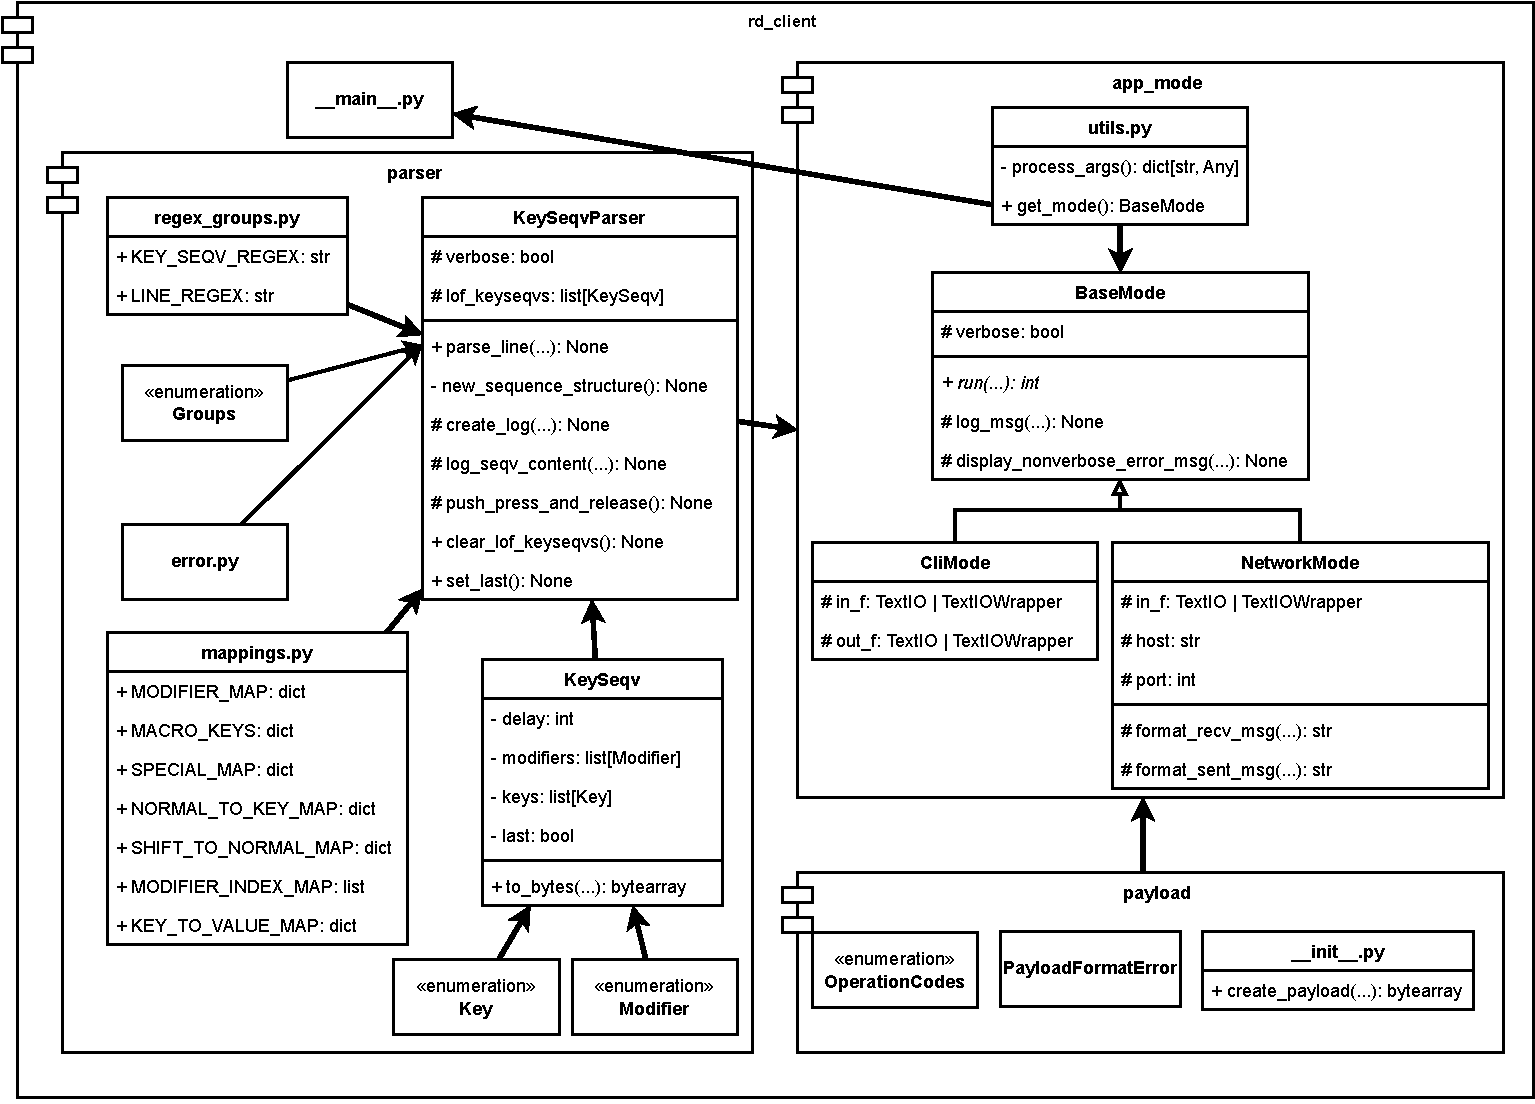
\includegraphics[width=\linewidth]{./obrazky-figures/rd_client_module.pdf}
    \caption{RD Client module UML class diagram.}
    \label{fig:rd_client_module}
\end{figure}

\section{Client application}
There are two modes to run the client application:
\begin{description}
    \item [CLI mode] is a CLI application that was made for creating static payloads. It converts the keystrokes written in Rubber Ducky language to a C source code. The user can use it to replace the existing \verb|rubber_ducky/keyseqv/key_seqv_script.c| file.
    \item [Network mode] is a CLI application that was made for updating the payload on the USB device wirelessly using sockets.
\end{description}
Both frontend applications classes (\verb|CliMode| and \verb|NetworkMode|) derive from that base class \verb|BaseMode| as seen in \autoref{fig:rd_client_module}. They both process the input script the same way by creating an instance of \verb|KeySeqvParser| class and feeding it with the input data as described in the previous section. What differentiate them apart is how they handle the processed data. \verb|CliMode| generates a new C source code file on the \verb|STDOUT| or output file if it was given. \verb|NetworkMode|, on the other hand, creates a TCP connection with the server and performs a series of requests where it sets the USB device to \emph{read-write} mode, sends \verb|PUSH_DATA| requests for each key sequence stored in \verb|KeySeqvParser|, set the device back to \emph{read-only} mode, and finish it off by sending a \verb|RUN_SEQUENCES| to start executing the payload. The \todo{diagram} shows the described steps.

The user can choose what mode to run based on the given application parameters. \verb|-n/--network| flag will toggle the \emph{network mode}. Otherwise, a \emph{CLI mode} is run by default. All of this is handled in \verb|get_mode| function in \verb|utils.py| (shown in \autoref{lst:get_modes}). Lastly, the user can also toggle an option to generate logs by adding \verb|-v/--verbose| flag. That is handled using Python's standard \verb|logging| library.

\lstset{
    caption={This snippet of code shows how the frontend mode is chosen.},
    label={lst:get_modes},
    language=python,
}
\begin{lstlisting}
# module rd_client.app_modes.utils

def get_mode() -> BaseMode:
    """Factory function that returns AppMode based on given arguments."""

    args = __process_args()

    # return selected mode
    if args['network']:
        # communication with RubberDucky using network (wifi)
        return NetworkMode(args['input'], args['port'],
                           args['host'], args['verbose'])
    # cli script parsing to C-file source code
    return CliMode(args['input'], args['output'], args['verbose'])
\end{lstlisting}

\section{Summary}
The diagram below \todo{add diagram} summarizes how the Rubber Ducky and client application work.

\chapter{Implementation evaluation}
\label{capabilities}
This section describes I will briefly evaluate my implementation of the Rubber Ducky device. When we connect our device to the machine the operating system immediately recognizes it as a composite device and the file system is correctly mounted (shows both "Automata.txt" and hidden ".README.md" files). We can check it by opening Device Manager on Windows (or running \verb|lsusb| command on Linux systems). The Vendor ID and Product ID of the device can be seen in \autoref{fig:device_manager_all}. Both values corresponds to the values specified in \verb|usb_descriptors.c| source file.
\begin{figure}[ht]
    \centering
    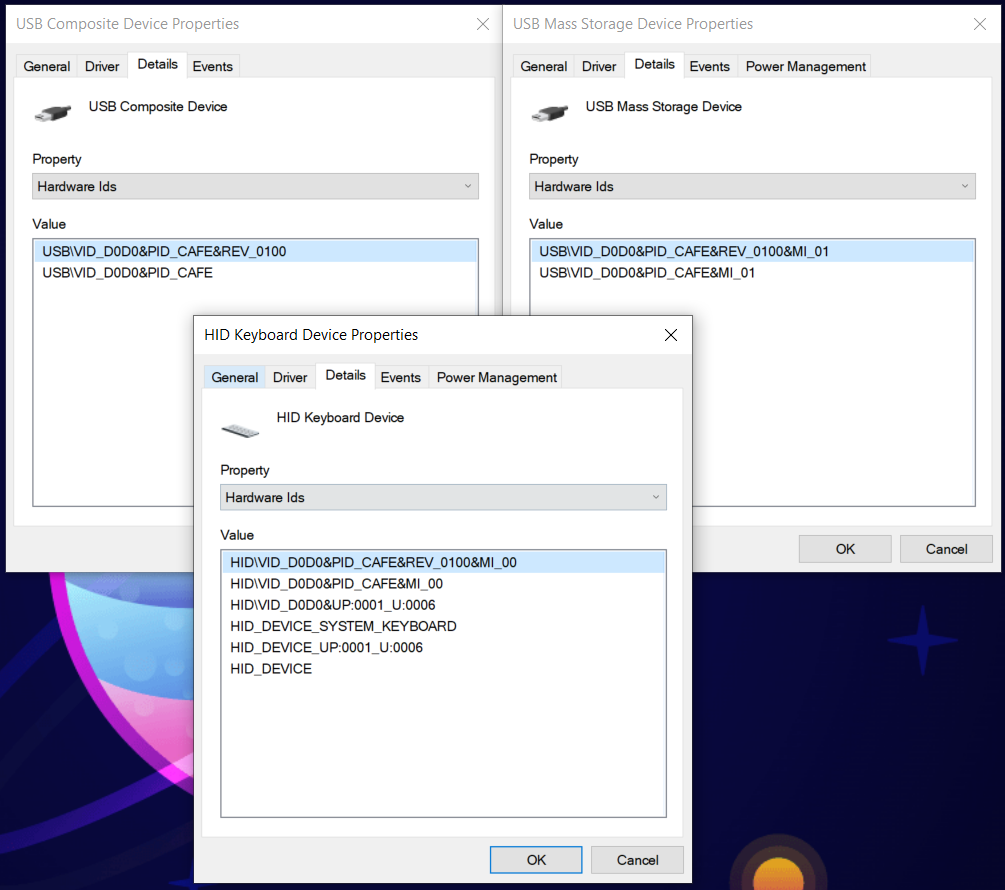
\includegraphics[width=0.75\linewidth]{./obrazky-figures/device_manager_all.png}
    \caption{Composite device info in Device Manager. \texttt{0xD0D0} value for Vendor ID and \texttt{0xCAFE} value for Product ID.}
    \label{fig:device_manager_all}
\end{figure}

The algorithm used to generate the payload is designed to produce as few key sequences as possible (if possible, it will send 6 keys at once). Based on the \verb|KEYPRESS_DELAY_MS| constant, we can test how fast and accurate can the device type. This was tested using the TUI application \verb|tt|\footnote{Link to the web page: \url{https://github.com/lemnos/tt}}. We prepared two test payloads: one with a regular 3 paragraphs long Lorem Ipsum text (2884 characters) and the other with a randomized list of printable ASCII characters (2800 characters)\footnote{Both payloads can be found here: \todo{url to them}}. The mass storage was disable for this test case. The \autoref{tab:typing_test} below shows an average typing speed of 20 tests.
\begin{table}[ht]
    \centering
    \begin{tabular}{|c|c|c|c|c|} \hline
        \multirow{2}{*}{\texttt{KEYPRESS\_DELAY\_MS}} & \multicolumn{2}{|c|}{\textbf{Lorem Ipsum}} & \multicolumn{2}{|c|}{\textbf{Randomized text}} \\ \cline{2-5}
                                                      & \textbf{WPM} &           \textbf{Accuracy} & \textbf{WPM} &               \textbf{Accuracy} \\ \hline
                                                    0 &       6590.8 &                   99.719 \% &      2625.05 &                      93.607 \%  \\ \hline
                                                   10 &       2641.1 &                   99.957 \% &       1128.5 &                     99.6285 \%  \\ \hline
                                                   20 &       1321.5 &                   99.981 \% &        566.1 &                      99.942 \%  \\ \hline
                                                   50 &       528.95 &                  99.9985 \% &          226 &                         100 \%  \\ \hline
                                                   80 &       329.95 &                      100 \% &          141 &                         100 \%  \\ \hline
    \end{tabular}
    \caption{Typing speed based on the \texttt{KEYPRESS\_DELAY\_MS} constant value. Testing was conducted on \texttt{Fedora Linux 36 (Thirty Six); kernel 6.2.9} operating system with AMD Ryzen 7 4700U process and 16GB of RAM.}
    \label{tab:typing_test}
\end{table}
We can see that the device's accuracy decreases at it types faster. Our Rubber Ducky device struggled a lot on Fedora system when executing the randomized text at the highest speed, with an average accuracy of less then 94 \%. The device made most of the mistakes when the Shift key modifier was not properly turned on or off. The table also shows that that randomized text slowed typing speed by approximately 2.3 times.

Lastly, we evaluate how accurate the delay feature of our device is. We use \verb|time| program, which is available on most Linux operating systems. Our device executes a \verb|time sleep 10| command in the shell, waits 2 seconds, and then terminate \verb|sleep| command with \verb|Ctrl+C| key shortcut. The time result is then appended to the output file. We repeat the test 20 times and average the results. What we ended up with is a rough estimate of our wait time. According to the result, the average time between starting and terminating the \verb|sleep| program was 2.02s. We can declare that the wait time of our device is accurate to 2 hundredths of a second.

\chapter{Malicious payloads}
\label{maliciousPayloads}
The chapter analyzes types of payloads that can be installed on our USB device, specifically the ones that were designed to cause some damage on the victim's machine. Most of the attacks require access to the command line application (or terminal). Here are a few example of payload's notion once the access to the command line has been granted:

\begin{itemize}
    \item update victim's system configuration,
    \item download and execute a malicious script from the internet or stored inside the connected device,
    \item perform a Denial of Service or BSoD (Blue Screen of Death),
    \item open a fake website to capture victim's username and password,
    \item create a communication backdoor by initializing a reverse shell.
\end{itemize}

The first on the list is \textbf{updating system configuration}. The attacker can create a payload that would for example change the network settings like changing the IP address of DNS server to redirect request to attacker's location, disable an anti-virus program, firewall, or built-in hardware such as a touchpad or keyboard.

Another possible attack is to simply download a malware from the internet and run in on the victim's computer (or run it from the mass storage). An example can be keylogger software. \textbf{Keylogger} is a program which run in the background and its task is to capture anything the user type with its keyboard. The captured keystrokes can be uploaded to the remote server controlled by the attacker. The attack can then analyze received data and extract user's login credentials. Keyloggers can be either software program or physical device (for example KeyGrabber\footnote{\url{https://www.keelog.com/keygrabber-keylogger/}}).

\todo{https://www.bleepingcomputer.com/news/security/fbi-hackers-use-badusb-to-target-defense-firms-with-ransomware/}

The attack can also create a payload which would perform a \textbf{Denial of Service} attack or execute a \textbf{Blue screen of Death} or \textbf{kernel panic}.


The attack can also force Blue Screen of Death or perform Ping of Death.

\todo{it can create a communication tunnel initializing a reverse shell}

\chapter{Testing defense mechanisms}
\label{defense}
At the time of writing this thesis, there are many available defensive software on the internet. In this section, I describe how some of them work and whether my device was successful in breaking pass any of them. I used free open-source program USBGuard on GNU/Linux and Kaspersky Endpoint Security program on Windows 10.

\section{Selected programs}
\textbf{USBGuard}\footnote{\url{https://github.com/USBGuard/usbguard}} is a software framework for implementing USB device authorization policies. It was developed in 2015 and has been manage by Red Hat Inc. since then. It consists of two main programs: \verb|usbguard-daemon| and \verb|usbguard|. The former is a service that runs in the background and applies USBGuard policies to each USB device. The behavior of the service can be configured by editing \verb|usbguard-daemon.conf|. The latter is a command line interface that provides the user with a tool to update the USBGuard policies.

Before I started experimenting I needed to initialize the service. The instructions were very simple: generate an initial policy file using \verb|usbguard generate-policy| and then start the service with \verb|systemctl start usbguard.service|. It was critical to generate the rules before starting the service, otherwise, all USB devices would be blocked by the daemon once started. The program scans all the USB devices and hubs currently connected to the machine and sets their target to "allow" meaning they are all whitelisted on the host machine. The testing environment was \verb|Fedora Linux 36 (Thirty Six); kernel 6.2.9|.

The program that I chose for Windows operating systems is called \textbf{Kaspersky Endpoint Security}\footnote{\url{https://www.kaspersky.com/small-to-medium-business-security/endpoint-windows}}. It is a security application that provides computer protection against various types of threads, network or phishing attacks. It contains a list of protection components such as File Threat Protection, Web Thread Protection, system scan, and much more. What we are interested in is their \textbf{BadUSB Attack Prevention}. It works as follows: when a new USB device that emulates a keyboard is connected to the computer, the user receives a pop-up window where he/she has to type 4 digit number that is displayed on the screen from the connected device. The testing environment for this application was \verb|Windows 10 21H2|.

I tested both software in the following way:
\begin{enumerate}
    \item Enable only HID class on the Rubber Ducky device.
    \item Connect the device to the host machine with the installed and running application.
    \item Observe the application's behavior.
    \item Give the USB device access to the system and connect the device again.
    \item Enable MSC on the Rubber Ducky device.
    \item Connect the device again and observe if something has changed.
\end{enumerate}
The payload that is present on the USB device opens a terminal or Powershell and runs \verb|ls| command. I also added a feature where the LED on the board turns on when the device starts to execute the payload.

First, I tested the USBGuard software on Fedora. When I connected the Rubber Ducky device to the machine with USBGuard running, as expected, no keystrokes injection happened. In fact, the device did not finish the enumeration process because the LED did not turn on. The system registers that a new device has been connected but the application immediately blocked it as you can see in \autoref{fig:usbguard_device_blocked}. After I change the policy for this particular device the status changed to "allow" and the payload was executed. Unfortunately, the beginning of the command was trimmed and only \verb|ls| command was executed (a new terminal did not open).

\begin{figure}[ht]
    \centering
    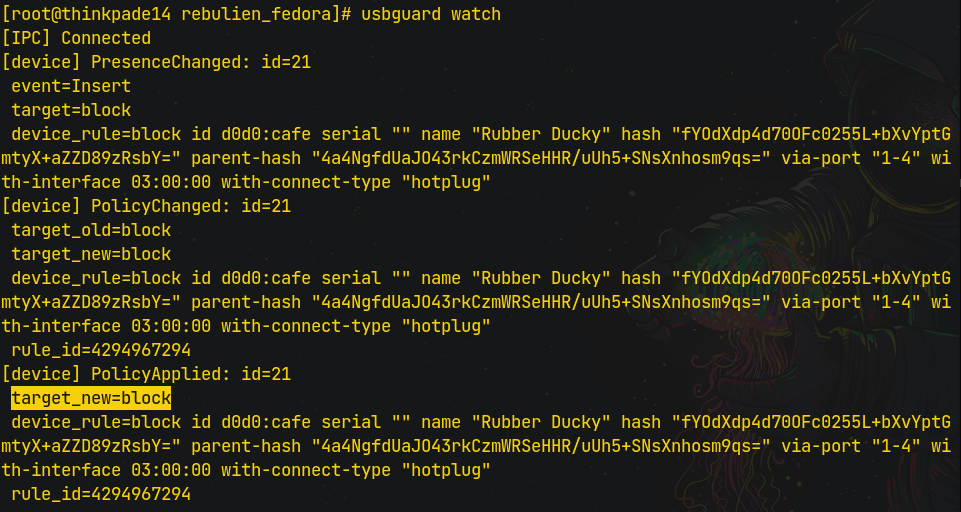
\includegraphics[width=\linewidth]{./obrazky-figures/usbguard_watch.png}
    \caption{Screenshot of USBGuard logging after a new USB device is plugged in.}
    \label{fig:usbguard_device_blocked}
\end{figure}

USBGuard also gave me the option to update the device's policy permanently. Once I whitelisted the Rubber Ducky device it did successfully fully execute the payload. I also tried to plug it into different ports. What I found was that the policy did not apply to the device if it was connected to a different USB HUB than previously \todo{show hub layout and explain it}. And lastly, I updated the device's firmware to enable MSC. And again the USBGuard successfully blocked the device and prevented it from executing the payload.

Kaspersky Endpoint Security program was next to be tested. Upon connecting the Rubber Ducky device I immediately received a pop-up window as shown in \autoref{fig:screenshot_kaspersky_popup}. The device did manage to execute the keystrokes but nothing happened on the host machine since it was "stuck" in the pop-up window. The Kaspersky program let me input the numbers using my mouse and whitelist the USB device.
\begin{figure}[ht]
    \centering
    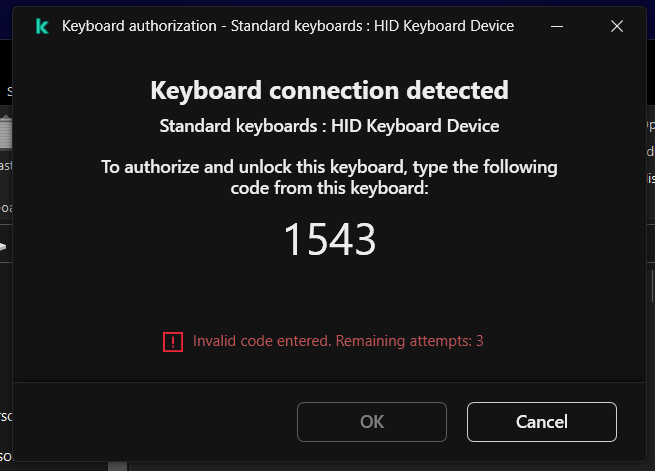
\includegraphics[width=\linewidth]{./obrazky-figures/kaspersky_keyboard_test.png}
    \caption{Pop-up authentication by Kaspersky Endpoint Security program.}
    \label{fig:screenshot_kaspersky_popup}
\end{figure}
Unfortunately, I was unable to locate the list of whitelisted devices to remove it from the list. Once the device was whitelisted it did successfully execute the payload just like on the previous test with USBGuard. But interestingly, unlike USBGuard, Kaspersky application did blocked all other ports including those within the same hub. And it also registered the change of firmware when MSC class was enabled. In \autoref{fig:kaspersky_report} you can see the reports of the program.
\begin{figure}[ht]
    \centering
    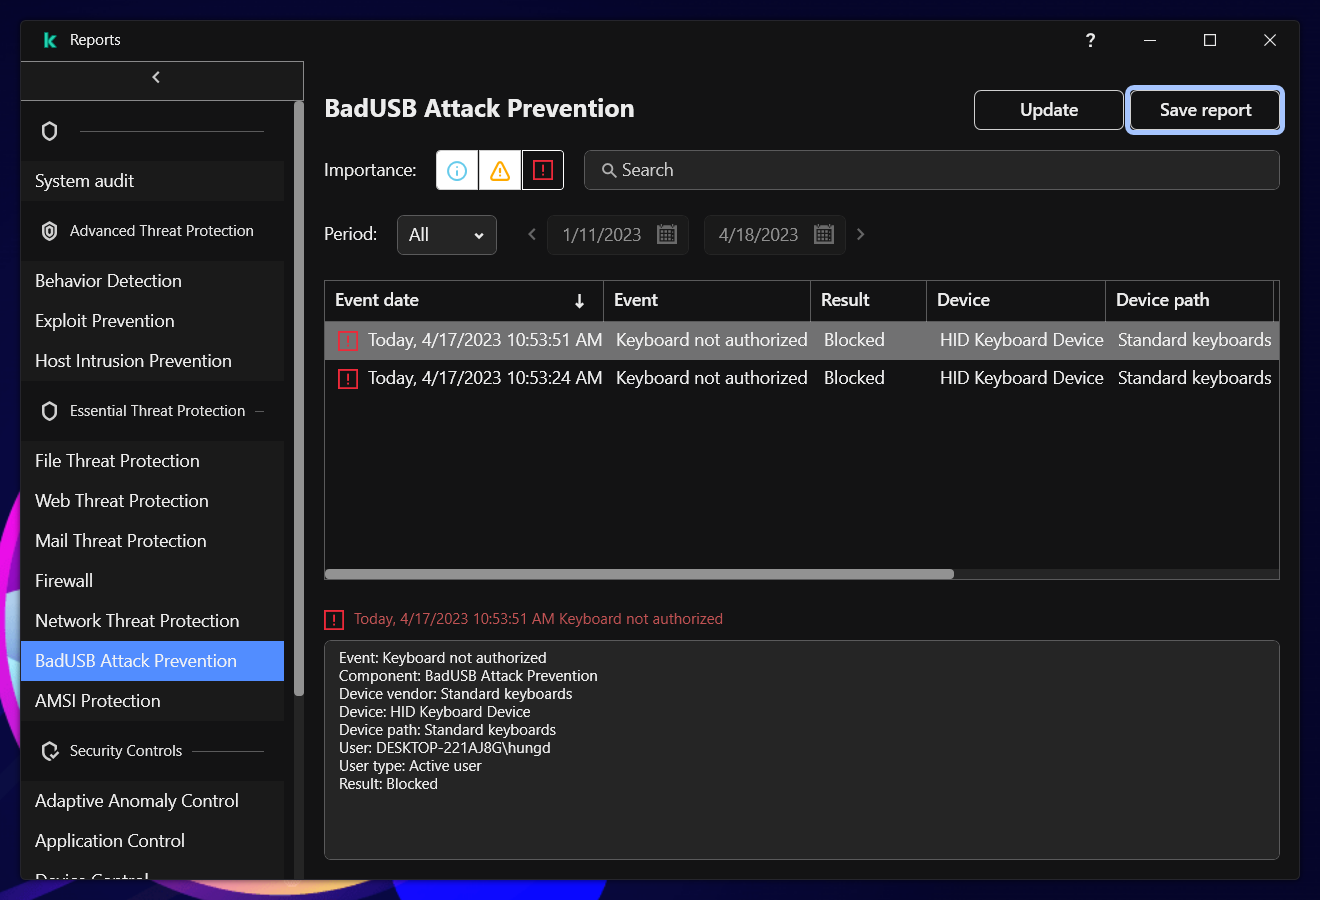
\includegraphics[width=0.9\linewidth]{./obrazky-figures/kaspersky_report.PNG}
    \caption{The Kaspersky Endpoint Security reports of the test. The reports are are sorted from the newest to the oldest. We can see that the first connection (at 8:02 PM) was blocked, then I authorized the device (8:12 PM), tried a different port (8:24 PM) and lastly plugged the device with an updated firmware into the first port (8:41 PM).}
    \label{fig:kaspersky_report}
\end{figure}

Both programs were very effective against the keystrokes injection attacks. The USBGuard was more effective since the device has no real access to the system and all USB related attacks would have been suppressed (not only the keystrokes injection attack). The disadvantage of USBGuard is its not very intuitive control. Most of the interaction are done using terminal since there is no official GUI application available. So unless the user is familiar with working with the command line, he/she cannot update a device policy\footnote{There used to be \texttt{usbguard-applet-qt} but this software is no longer supported. The latest project that provides a user-friendly notification pop-ups related to device presence update is \texttt{usbguard-notifier} (\url{https://github.com/Cropi/usbguard-notifier})}.

Kaspersky on the other hand gives the users a user-friendly GUI application together with online documentation. Unfortunately I was able to break through the defense by sending the authentication PIN through WiFi. So if the attack has an access to the screen, he will gain the access to the victim's machine. Another weakness of Kaspersky application is that it only covers keystrokes injection attacks. Other types of attacks (such as network cards spoofing) will not be detected.


\begin{figure}[ht]
    \centering
    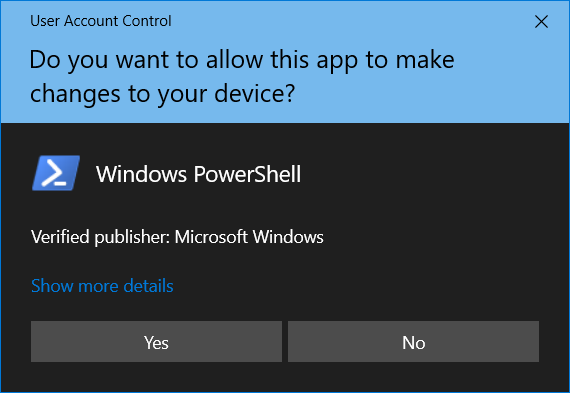
\includegraphics[width=0.4\linewidth]{./obrazky-figures/basic_notification.PNG}
    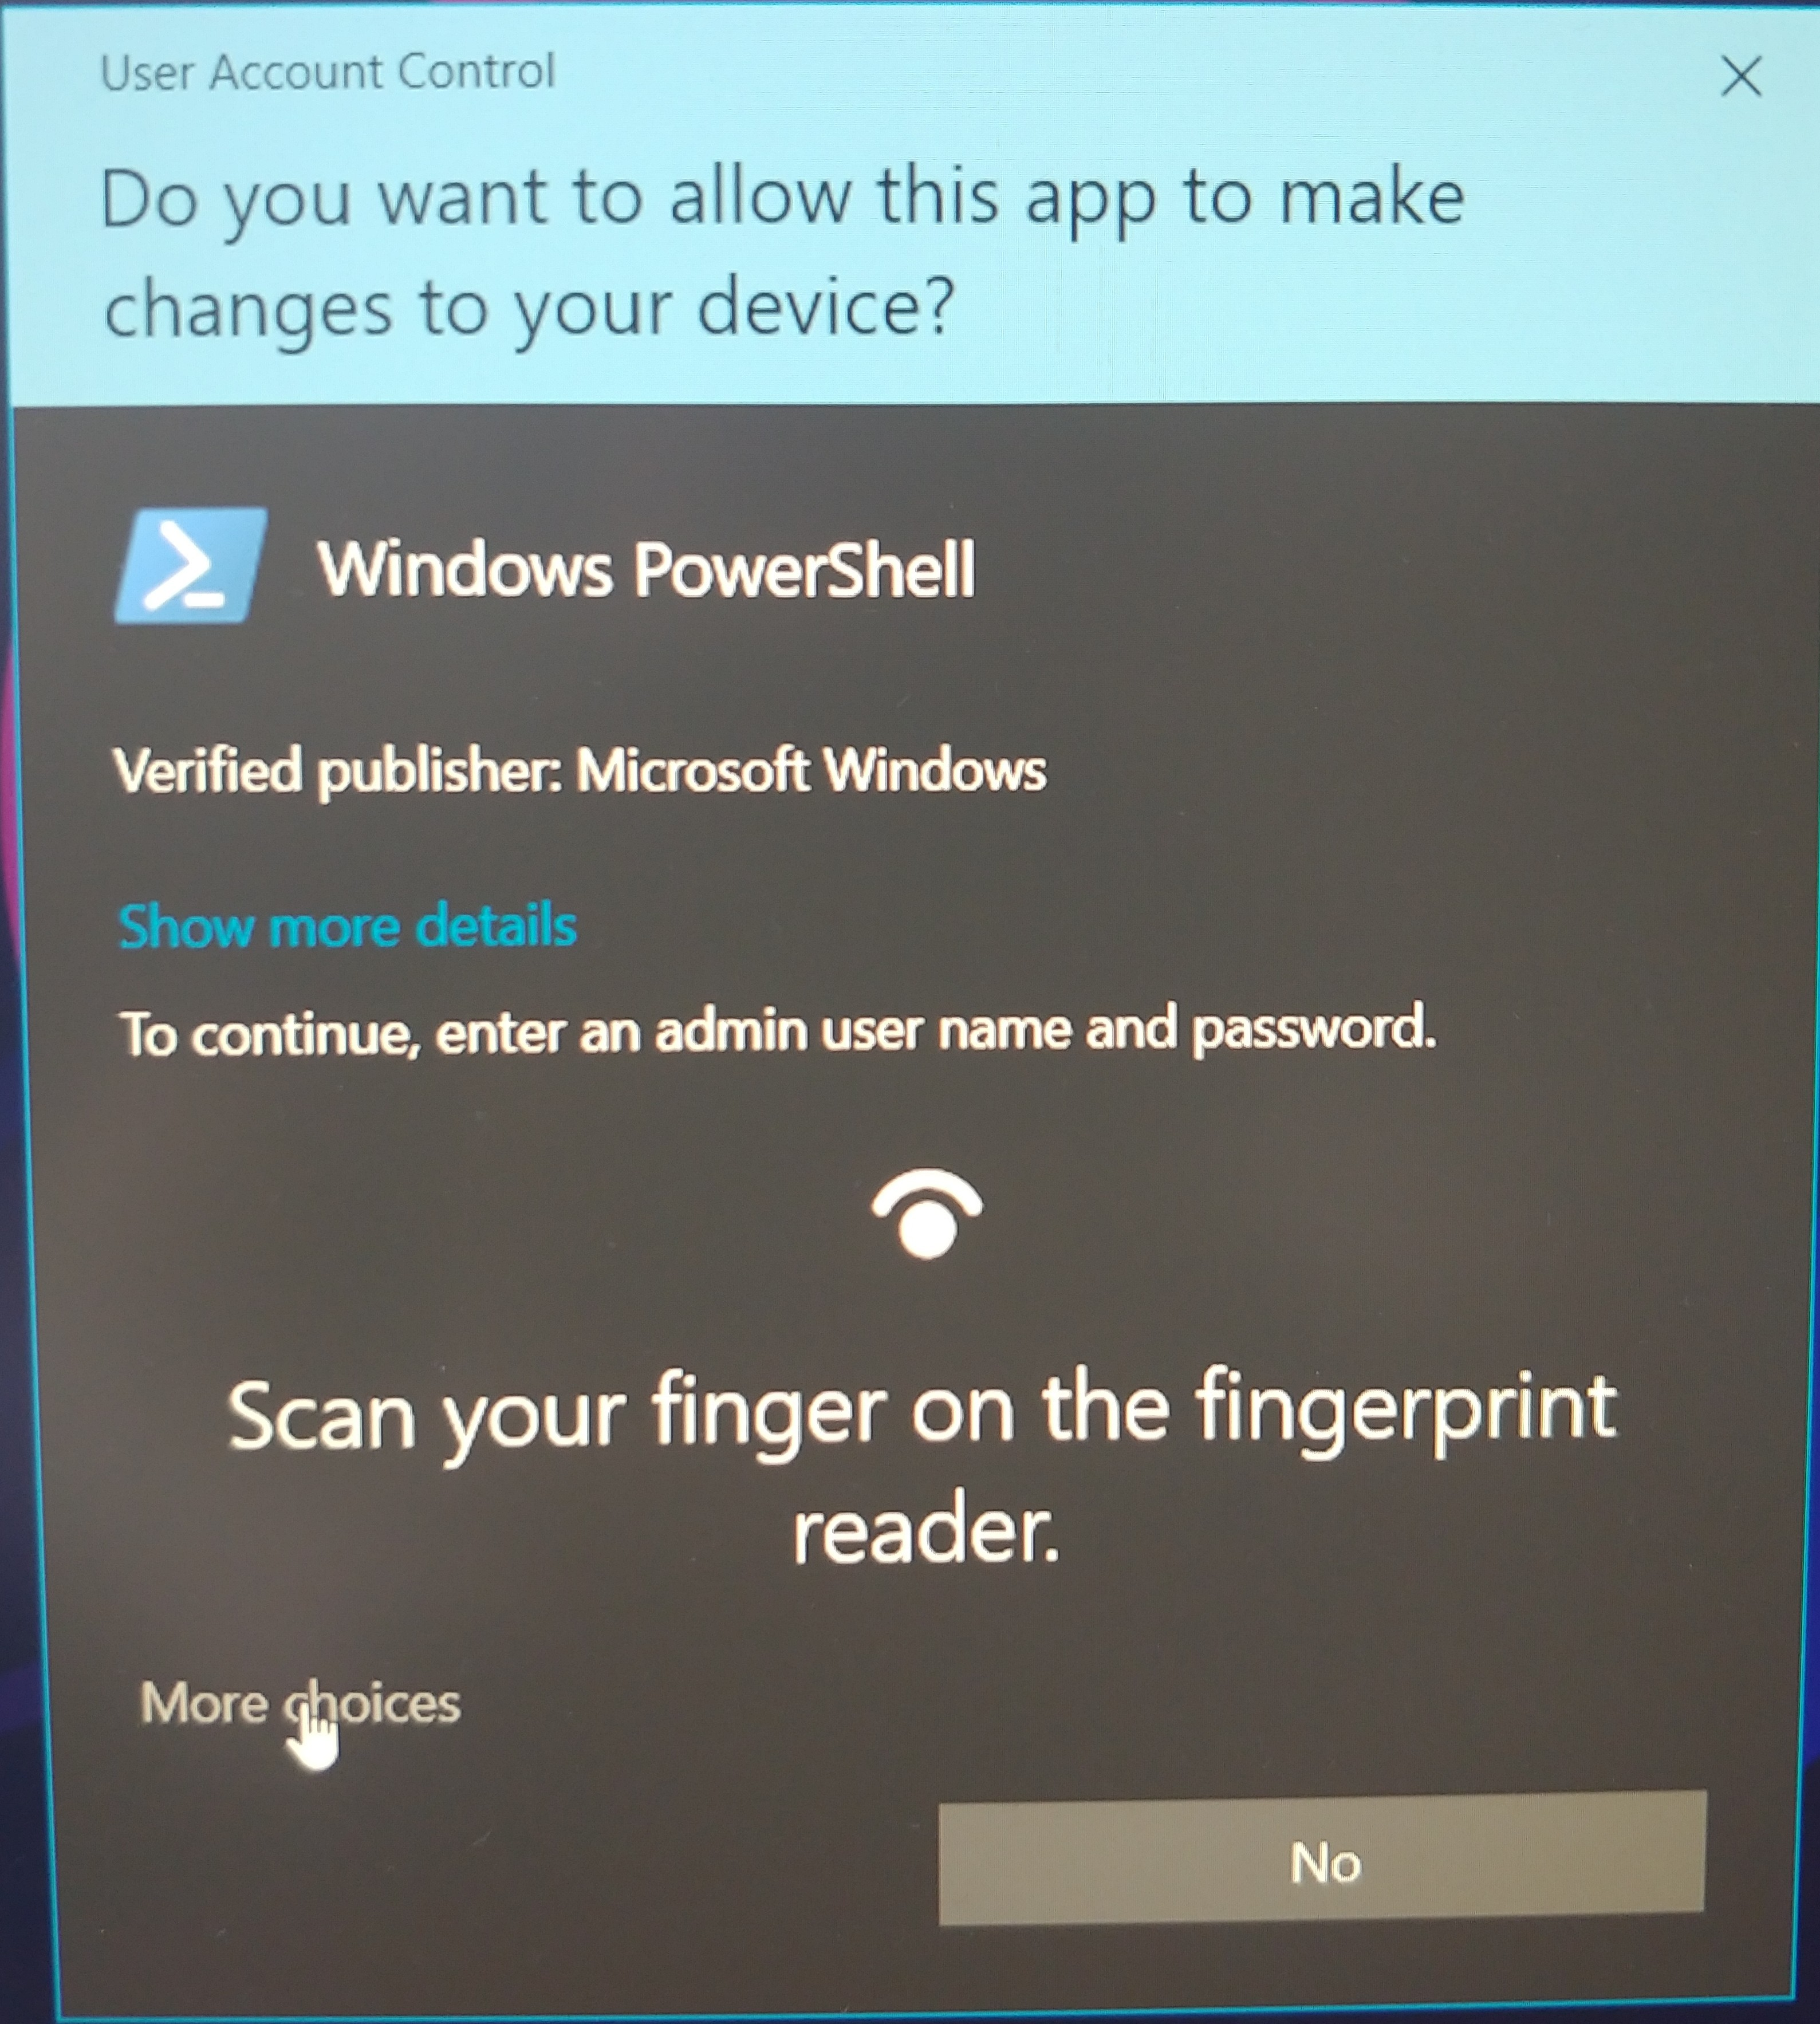
\includegraphics[width=0.4\linewidth]{./obrazky-figures/notification_with_authentication.jpg}
    \caption{The "run as administrator" pop-up window before (on the left) and after (on the right) the registry value update.}
    \label{fig:notifications}
\end{figure}

\section{Another defense mechanism available}
As stated in \autoref{maliciousPayloads}, most of the attacks requires an access to the terminal/command line. So another way to protect the host machine is by setting a password for running a command line as an administrator on Windows operating systems. All that is needed is to change the Windows registry\footnote{The instructions can be found here: \url{https://www.manageengine.com/device-control/badusb.html}}. The result can be seen in \autoref{fig:notifications}. As we can see before we updated the registry, it was fairly easy to open a terminal (or any other application) as an administrator as the only thing preventing us from doing so was a "Yes/No" confirmation buttons. But the new notification pop-up windows requires us to enter the user name and password (or any other type of authentication).

Another defense mechanism was presented in the work \cite{goodusb} by Tian and his team is called \textbf{GoodUSB} in 2015. They modified a Linux kernel module that maps USB devices to specific whitelisted drivers (for example an audio device such as headphones that is also registered as a Human Interface Device should only be able to execute a limited number of keys like \emph{Volume Up} and \emph{Volume Down}). Then they introduced a GoodUSB service (called gud) which sits in between the host controller and USB drivers. Upon connecting the USB device to the computer the user is asked to identify the device's functionality. If the device is marked as malicious GoodUSB service will redirected it to a virtualized USB honeypot where it can be monitored and analyzed. Otherwise, a driver will be loaded. The GoodUSB architecture can be seen in \autoref{fig:defense_mechanism_architectures}.

And last defense software that I will present here is \textbf{Cinch} which is a work by Sebastian Angel and his team from The University of Texas at Austin and New York University \cite{197175}. Their approach to USB attacks is to create a mediator between a hardware layer host controller and software layer HCI\footnote{Host Controller Interface, of HCI, is a register-level interface that enables a host controller for USB or IEEE 1394 hardware to communicate with a host controller driver in software. Link to the article: \url{https://en.wikipedia.org/wiki/Host_controller_interface_(USB,_Firewire)}}. The USB data are then transferred through a narrow choke point where it can be analyzed. The Cinch architecture can be seen in \autoref{fig:defense_mechanism_architectures}. Cinch uses I/O virtualization hardware to redirect \emph{direct memory access} and interrupts to a red virtual machine. The virtual machine then encapsulates and sends USB transfers through the Tunnel to another virtual machine (called Gateway) where it applies all security policies. Once finish, the USB transfer is then sent to the host's HCI (blue machine).
\begin{figure}[ht]
    \centering
    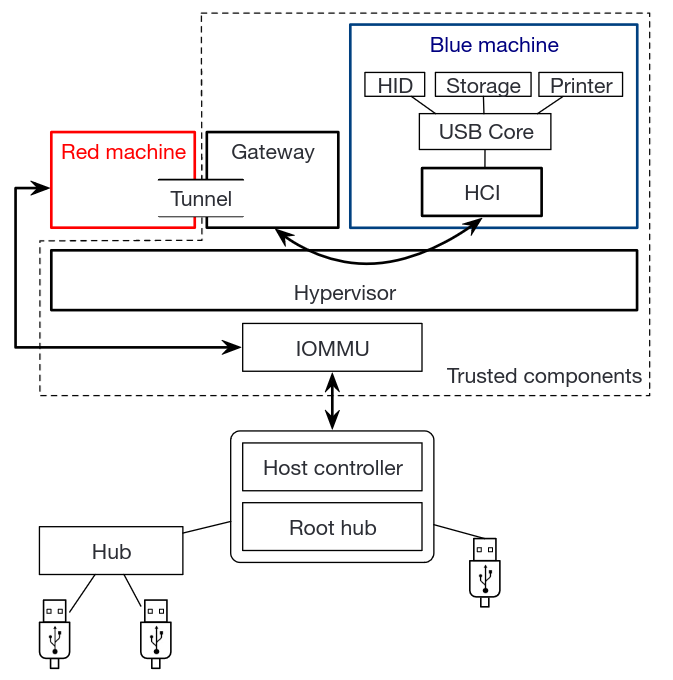
\includegraphics[width=0.4\linewidth]{./obrazky-figures/cinch_arch.png}
    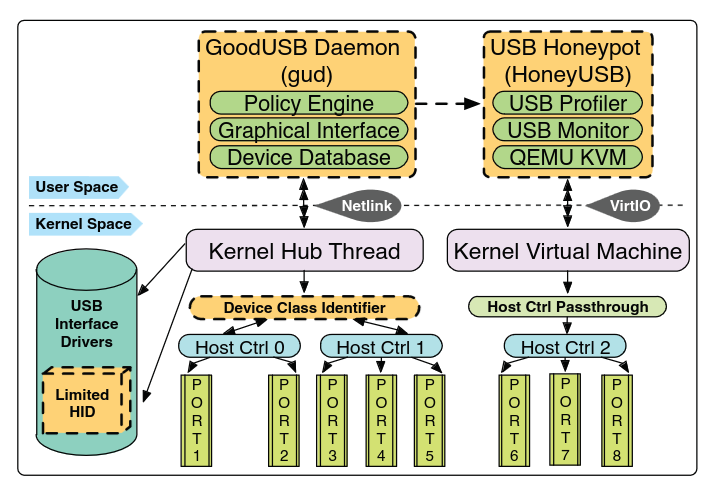
\includegraphics[width=0.4\linewidth]{./obrazky-figures/goodusb_arch.png}
    \caption{Cinch (left) and GoodUSB (right) architecture designs side by side. Both of these pictures were taken from their corresponding papers.}
    \label{fig:defense_mechanism_architectures}
\end{figure}

Other defense concepts are:
\begin{itemize}
    \item block the USB device when it starts typing with inhuman speed \cite{KerschbaumFlorian2018UBUK}, \cite{arghire_2020},
    \item disable firmware updates,
    \item disable USB drivers on host machine,
    \item hardware USB data blocker (also known as "USB condom")\cite{al-sibai_2023}
    \item and many more...
\end{itemize}
There is one concept which occurred me while I was writing this thesis and it is related to \autoref{customLanguage}. The notion here is that the majority of keystrokes injection payloads rely on the standard US QWERTY keyboard. So, if the operating system changes the keyboard layout, for example, to CZ DVORAK after connecting in a keyboard device, the payload will not be able to properly execute the payload because each key is mapped to a different output than on QWERTY. Of course, this is only a concept that has yet to be implemented. FuIt is also very insufficient since the attack will be successfully executed if the attacker guesses the keyboard layout that is set. Furthermore, it is insufficient because the attack will be successful if the attacker knows the keyboard layout that is set. And keyboard layouts only change printable keys, thus the attack will remain unchanged if the payload simply consists of modifier and non-printable keys (for example using \verb|Enter|, \verb|Tab| and arrow keys).

\chapter{Conclusion}
\label{conclusion}
% TODO:
